% Chapter4
\chapter{Implementierung} \label{chapter:thevetestcase}
\section{Modellierung der Anlage}
Für das Aufbauen einer Anlage ist ein vorab überlegtes Konzept von großer Bedeutung. Mittels des \ac{RI} wird ein schematisches Abbild der Apparatur erstellt. Die anfangs aufkommenden Änderungen ergeben sich angesichts der zeitlich bedingten, schrittweisen Implementierung der Anforderungen. Initial wird hoher Wert auf Redundanzen gelegt. Erst eine größere Anzahl an Bauteilen kann einen parallelen Ablauf mehrerer Arbeitsschritte ermöglichen. Durch die drei eingebauten Tanks und zwei Reaktoren, die mittels der drei Hauptleitungen verbunden sind, ist das Umfüllen zwischen zwei Tanks, sowie das gleichzeitige Befördern von Flüssigkeit vom dritten Tank in einen der Reaktoren möglich.\\

Die zwei Pumpen sind so platziert, dass bei einem auftretenden Defekt die andere Pumpe deren Aufgabe übernehmen kann. Arbeitsschritte können dadurch zwar nur noch sequentiell abgearbeitet werden, jedoch kommt es nicht gleich zu einem totalen Ausfall der Funktionalität der Anlage. Eine weitere Absicherung gegen möglich aufkommende Störfälle ist die Position der Tanks. Durch ihre Lokalisation an der höchsten Stelle der Apparatur besteht die Opportunität die Schwerkraft zu nutzen.\\

\begin{figure}[h!]
  \centering
  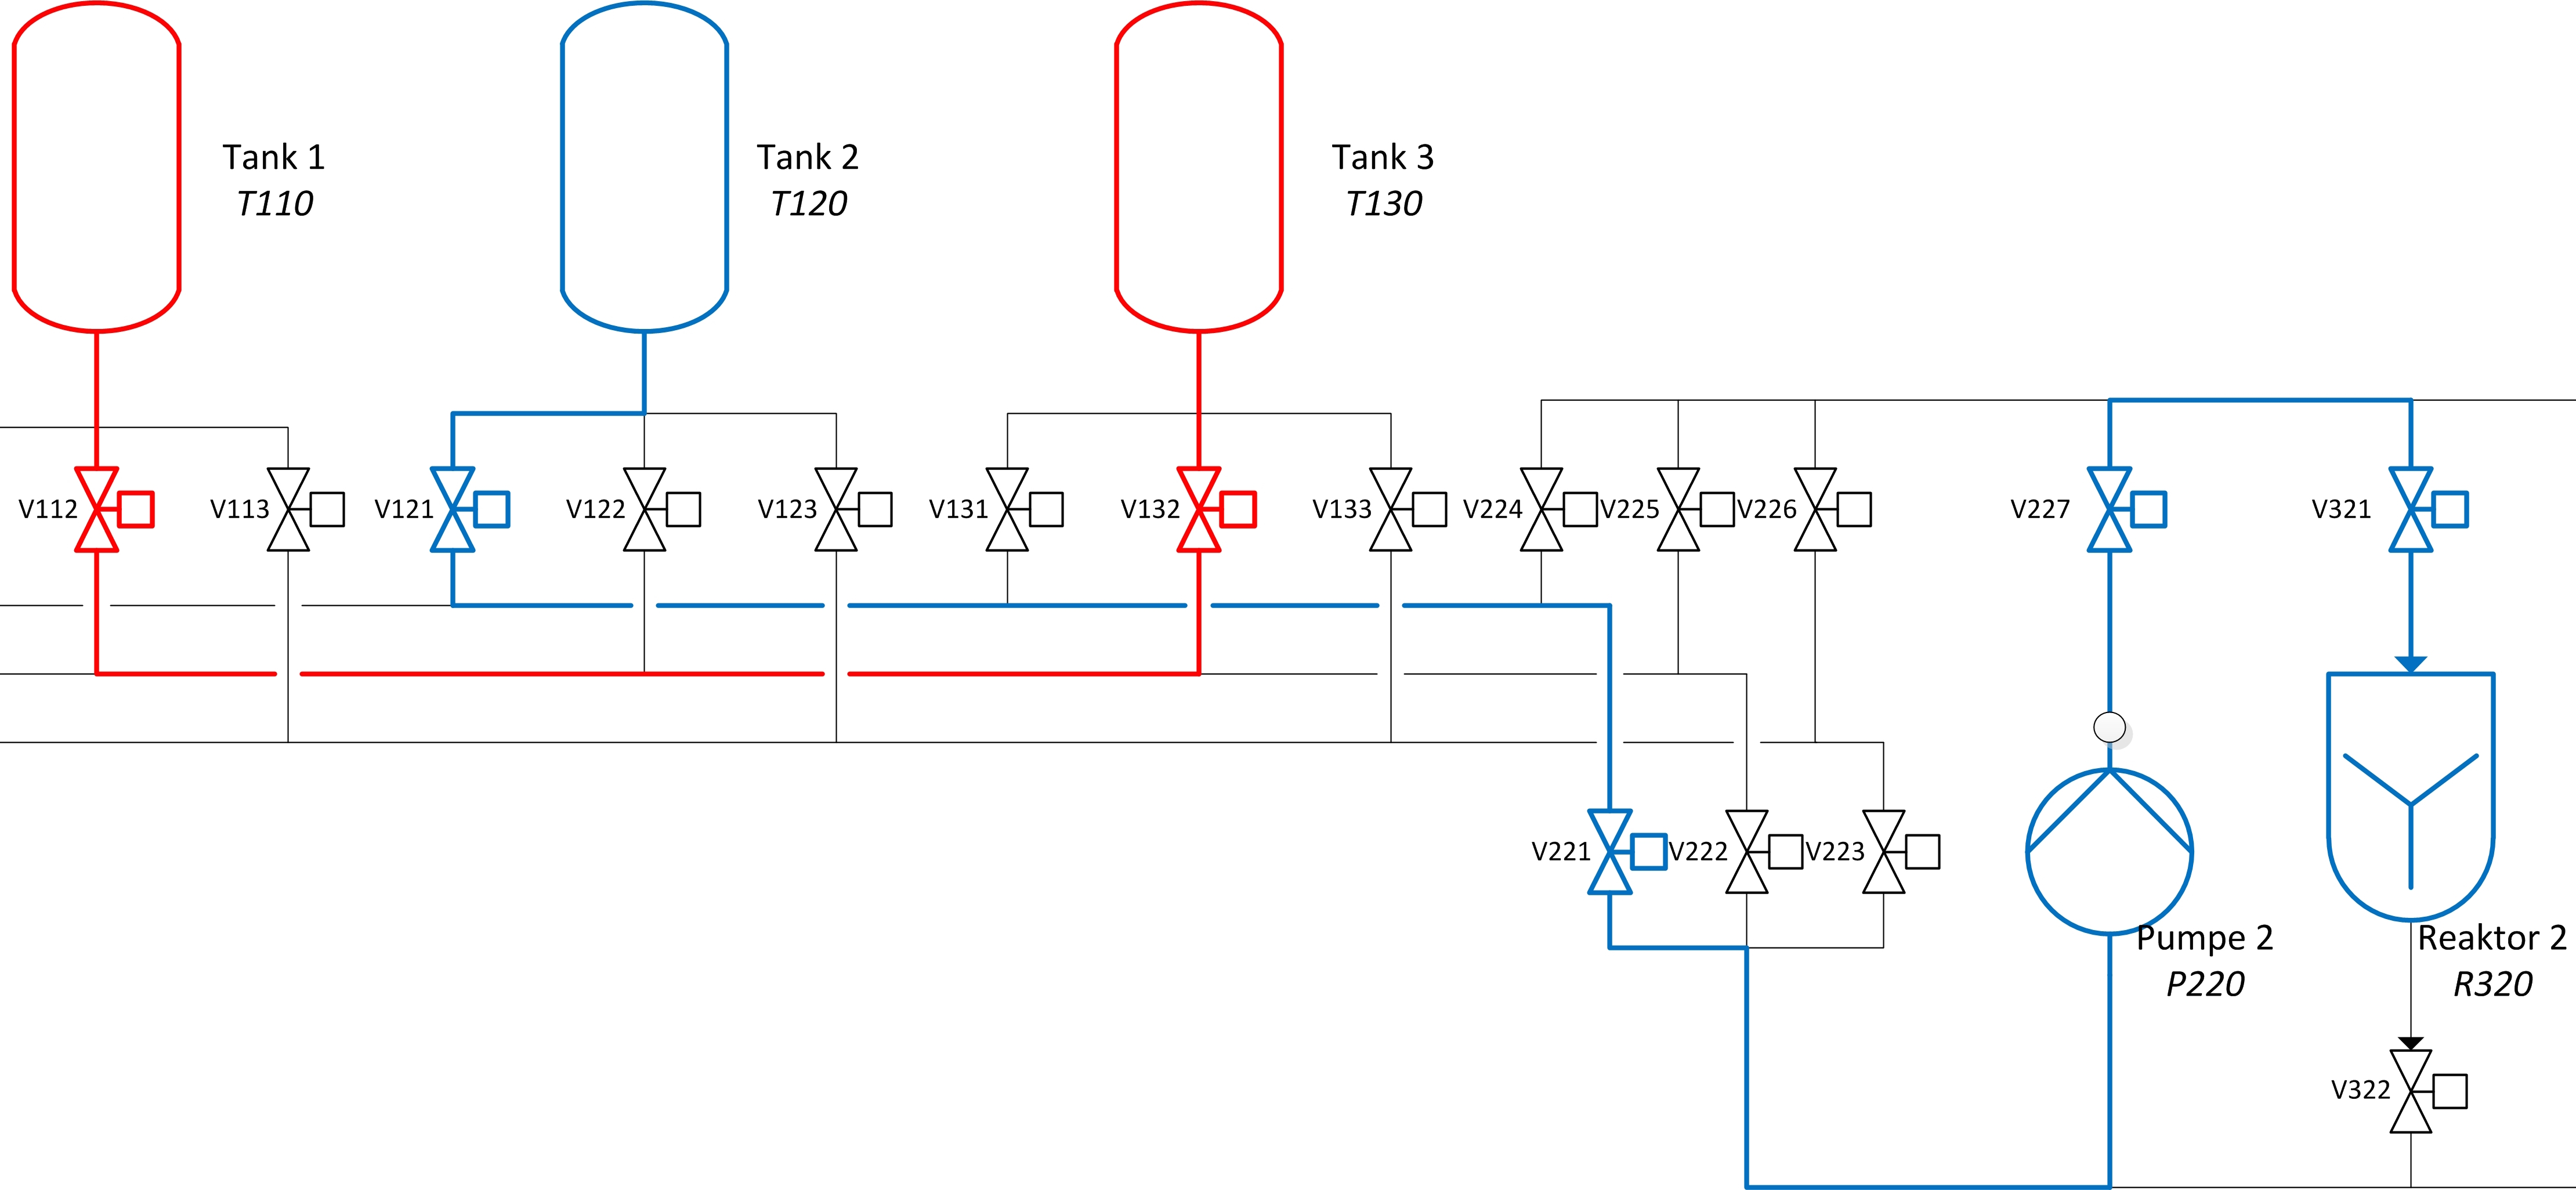
\includegraphics[width=1\textwidth]{graphics/implementation/RI_Impl_cropped.jpg}
  \caption{Mögliche Parallelität im \ac{RI}}
\end{figure}

Jedes Ventil hat eine vorteilhafte Durchflussrichtung, die meistens mit einem Pfeil direkt auf dem Bauteil gekennzeichnet ist. Ganz abgesehen davon, ob es sich um ein Ventil handelt, welches im stromlosen Zustand geschlossen ist oder ob es ein schließendes Ventil ist, diese Vorgabe sollte stets eingehalten werden. Aspekte wie dieser haben in die Modellierung der Anlage selbstverständlich eingebaut zu werden.\\

\begin{figure}[h!]
  \centering
  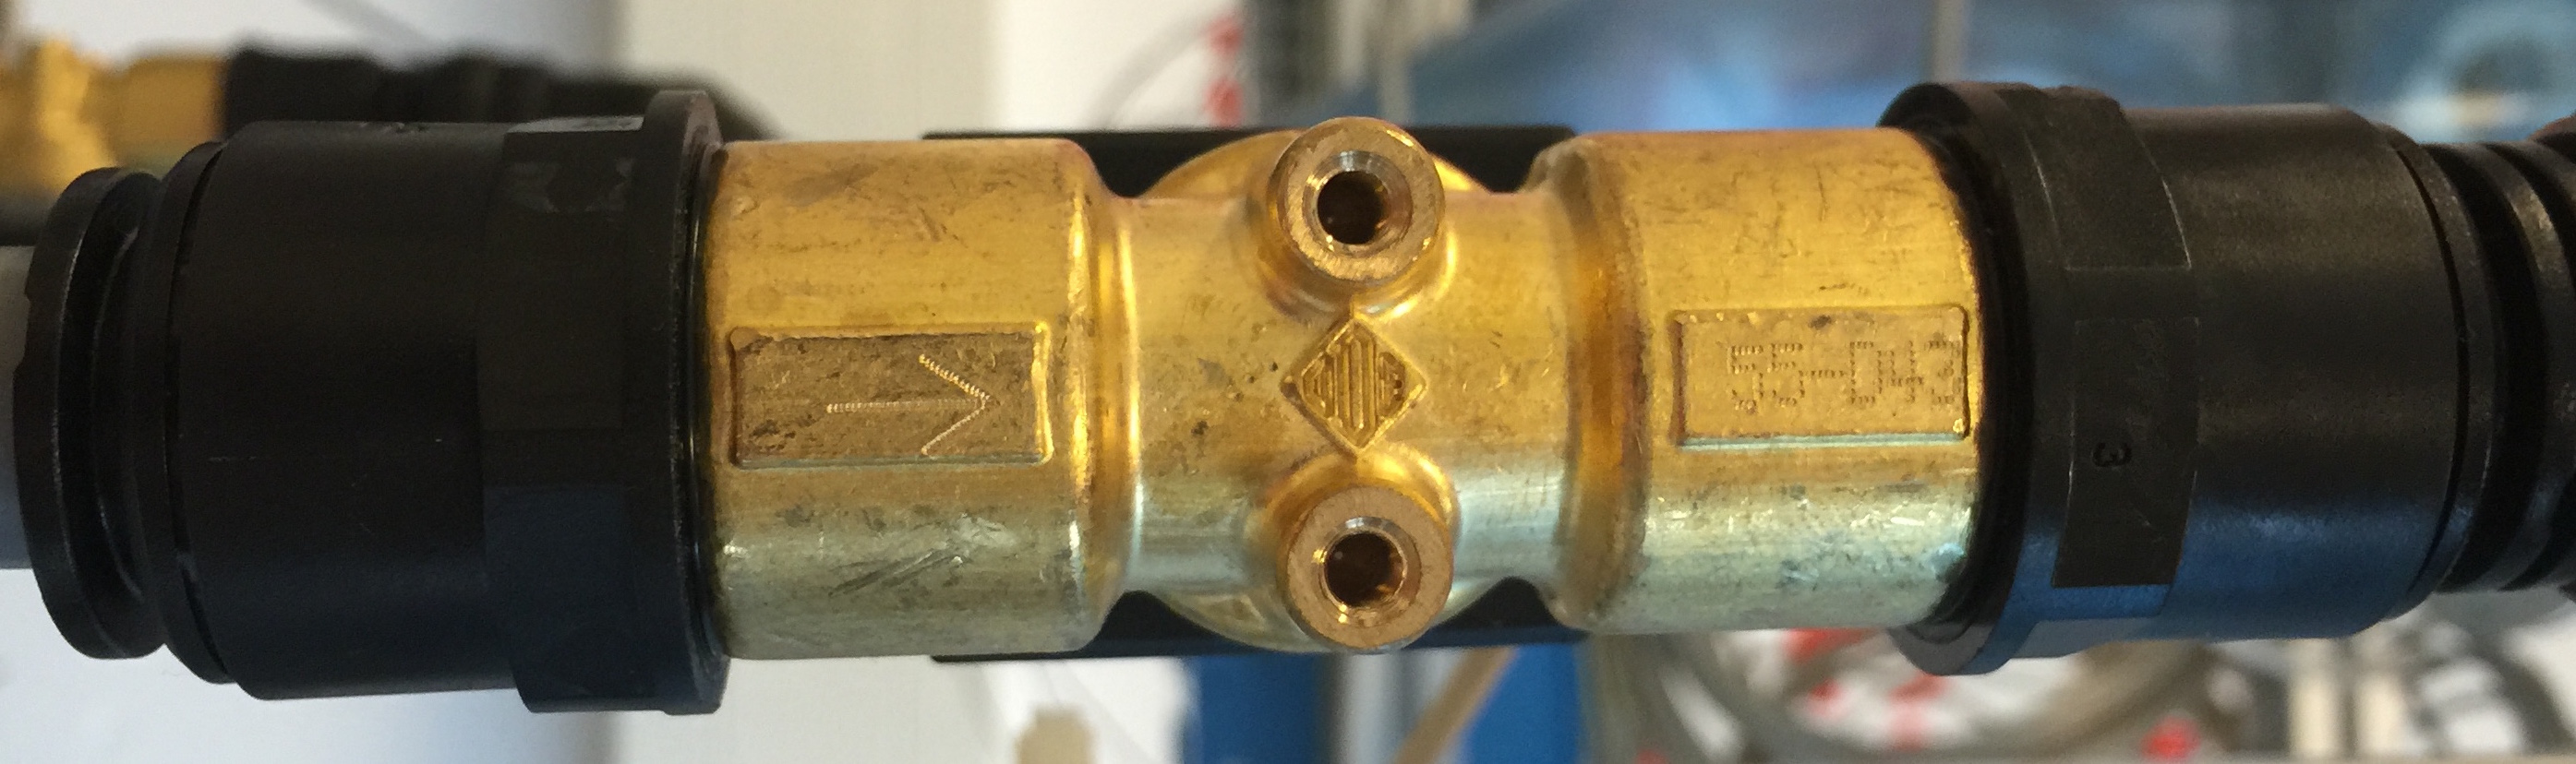
\includegraphics[width=0.7\textwidth]{graphics/implementation/Fliessrichtung.jpg}
  \caption{Ventil mit vorteilhafter Fließrichtung}
\end{figure}

Um in der Anlage befindliche Flüssigkeiten zu entfernen, muss ein eigens für den Auslass vorgesehenes Ventil installiert werden. Vorteilhafterweise handelt es sich bei der Position dieses Bauteils um den tiefsten Punkt der Apparatur. Alternativ dazu kann dieses auch direkt nach einer Pumpe montiert werden.

\section{Aufbau der Anlage}
Auf Basis des \ac{RI} kristallisiert sich eine exakte Anzahl an benötigten Bauteilen heraus. Für den noch bevorstehenden Aufbau der Anlage ist zu beachten, dass beim Auswählen der Einzelteile alles kompatibel sein muss. Nicht vorhandene Vereinbarkeit kann vor allem für diesen speziellen Anwendungszweck zu katastrophalen Auswirkungen führen, da einerseits mit Flüssigkeiten gearbeitet wird, sowie gleichzeitig stromdurchflossene Leitungen existieren. Eine Verbindung dieser genannten Komponenten hätte irreparable Schäden zur Folge. Im Rahmen einer übergeordneten Forschungsarbeit wurde diesem Projekt ein Budget von \euro6000.- zugesprochen. Die Auswahl der benötigten Teile hat verständlicherweise im Rahmen dieser Geldmittel zu geschehen.\\
	
	Für einige verwendete Element gibt es spezifische Parameter, die auf jeden Fall einzuhalten sind:\\
	
	\textbf{Ventile:}\\
	Ein ausschlaggebendes Kriterium der verwendeten Ventile ist, dass sie in stromlosem Zustand geschlossen sind. Im Falle eines Ausfalls der Energieversorgung kann somit sichergestellt werden, dass sich alle Verbindungen aus Schutz vor Flüssigkeitsverlust schließen. Für die Funktion der Nutzung der Schwerkraft zum Umleiten von Flüssigkeiten ist auch relevant Ventile zu haben, die keinerlei Vordruck benötigen um den Durchfluss zu gewähren.\\

	\textbf{Tanks:}\\
	Abgesehen von einem für Testzwecke vernünftigen Füllvolumen ist es erforderlich einen Tank zu wählen, dessen Ausgang sich am niedrigsten Punkt befindet. Andernfalls kann man nur bedingt Nutzen aus der Schwerkraftsteuerung ziehen.\\
	
	\textbf{Pumpen:}\\
	Mit Hilfe eines Gleichstrom - Wandlers muss es möglich sein, die Pumpen mit dem zur Verfügung stehenden Ausgangstrom der \ac{SPS} von 0 bis 10 Volt zu betreiben.\\
	
	\textbf{Rohre:}\\
	Die Rohre müssen jedenfalls dem Druck der Pumpen standhalten können. Desweiteren ist das exakt abzustimmende Einpassen in die Ventile, um Dichte gewährleisten zu können, ein wichtiger Parameter.\\

	Die bereits bei der Bestellung bekannten, tatsächlichen Maße der Bauteile, hatten einen relevanten Einfluss auf den finalen Aufbau. Da es auch bei der Profilplatte physikalische Grenzen gab, musste die endgültige Positionierung genauestens überlegt ausfallen. Der zukünftigen Vereinfachung des Aufbaus der Produktionsanlage, wurde projektintern beschlossen, ein kleines Modell der Apparatur zu erstellen. Da aus einem \ac{RI} keinerlei Information zur endgültigen Lokalisation der Bauteile ersichtlich ist, wurde ein erster physikalischer Prototyp konstruiert. Mit Hilfe diesem konnten Abstände zueinander stehender Elemente deutlich gemacht werden. Realisiert wurde der genannte Prototyp mit leicht zugänglichen Arbeitsmaterialien wie etwa Trinkhalme, Papier und Klebeband.\\

	Für den tatsächlichen Aufbau ergab sich günstigerweise die Möglichkeit, mechanische Anforderungen mit Hilfe der technischen Werkstätte abzuwickeln. Profilschienen, die als stabilisierendes Gerüst dienten, wurden penibelst mit der Aluminiumsäge auf das gewünschte Maß geschnitten. Im späteren Verlauf ergaben diese samt den Tanks den ersten aufgebauten Teil der Anlage. Für die Verbindung der Tanks, Pumpen, Ventile und Reaktoren dienten undurchsichtige Kunststoffrohre. Um gewährleisten zu können, dass die Verbindung dicht ist, mussten die Rohre unbedingt gerade geschnitten sein. Abermals durften dafür Maschinen der mechanischen Werkstatt verwendet werden. Erst mit einer Bandsäge grob vorgeschnittene Rohrstücke wurden in eine konventionelle Drehmaschine eingespannt. Mit einem scharf angeschliffenen Drehstahl war es anschließend möglich, den unsauberen Schnitt absolut plan zu gestalten. Nachdem abschließend einzelne Komponenten noch entgratet wurden, war die Arbeit an den Rohren zur Verbindung getan.\\
	
	\begin{figure}[h!]
	  \centering
	  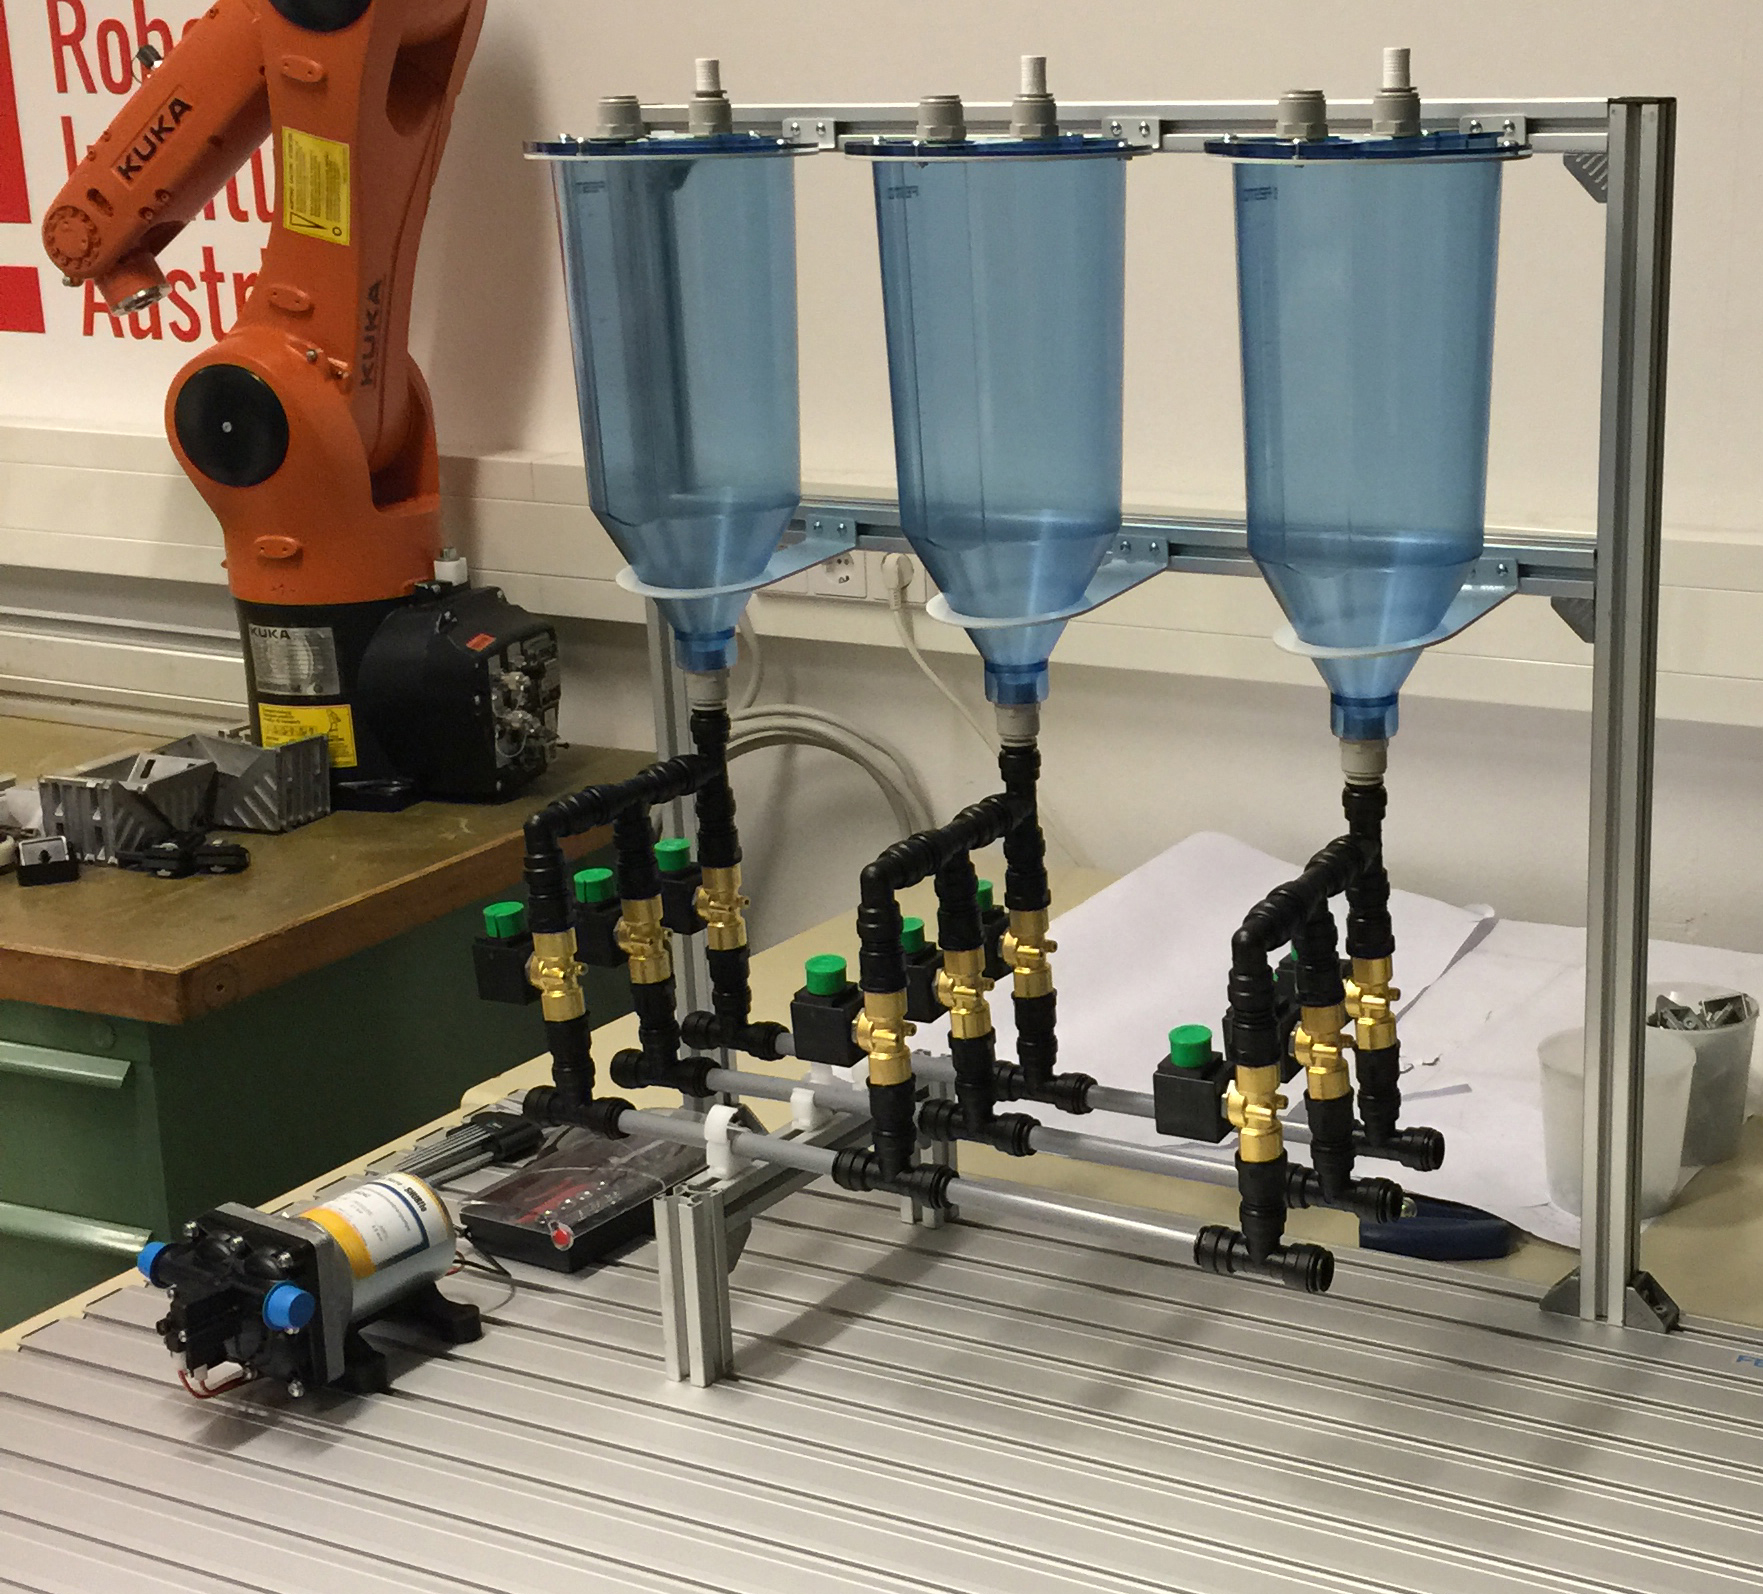
\includegraphics[width=0.8\textwidth]{graphics/implementation/ErsterAufbau.jpg}
	  \caption{Erster Aufbau der Anlage}
	  \label{fig:erster_aufbau}
	\end{figure}	
	
	Verbindungen mit den ersten neun Ventilen der Hauptleitungen und den Tanks konnten ab sofort verlegt werden.\\
		
	Das Einbauen der bestellten Pumpen gestaltete sich komplizierter als gedacht, da die ursprüngliche Bestellung einen Fehler beinhaltete. Nur eines der beiden gelieferten Modelle entsprach der gestellten Anforderung, was einschließlich der Rücksendung weitere wertvolle Zeit kostete. Unterdessen konnte die zweite Pumpe verbaut werden. Funktionale Bauteile dieser Art mussten bei der zeitgemäßen verfügbaren Leistung gut gedämpft werden. Angesichts der Tatsache, dass man mit dieser Pumpe bis zu 30 Meter hoch pumpen könnte, befindet sich auf der Unterseite ein gummiertes Verbindungsstück, um bei Inbetriebnahme die stärksten Vibrationen abfangen zu können. Mit vom Profilschienen Schneiden übergebliebenen Reststücken wurde eine Konstruktion gebaut, um die Höhe der Pumpe mit der der Rohre gleichzusetzen. Unmittelbar nach der Pumpe wurde ein Durchflusssensor angebracht, der im späteren Verlauf des Projekts zur automatischen Steuerung beitragen sollte.\\\\
	Abermals in der Werkstatt genauest zugeschnittene Profilschienen ergaben eine Konstruktion zur Aufhängung der Reaktoren. Das beste Beispiel der Bauteil-Positionsuntreue eines \ac{RI} war anhand des aufkommenden Arbeitsschritts zu sehen. Ursprünglich waren die beiden Reaktoren seitlich der restlichen Anlage platziert. Da es die Profilplatte aber nicht zuließ, da sie nur eine gewisse Breite hatte, mussten diese in den Vordergrund geholt werden. Bei der Bauart der Reaktoraufhängung war zu beachten, dass das größt möglich aufkommende Gewicht ausschließlich dort zustande kommen konnte, da Reaktoren zum Mischen mehrerer Tankinhalte verwendet werden können. Diese Überlegung musste jedenfalls dazu beitragen, ausreichend Stabilität und Belastungsfähigkeit zu erlangen.\\\\
	Die bereits eingebauten Ventile besaßen jeweils zwei Anschlussleitungen für das Signal und ein Schutzleiter. Die Verkabelung selbst wurde mit einem starren Leitern mit drei Adern umgesetzt. Aus Gründen der Übersichtlichkeit wurde jedes Kabel sowie Ventil beschriftet, um eventuell aufkommende Komplikationen zu unterbinden. In den Rillen der Profilschienen verlegt, wurden alle mit Kabelbindern verbundenen Leiter zur \ac{SPS} zurückgeführt. Im späteren Verlauf eines Folgeprojekts sollte eine Verlegung der \ac{SPS} an die Unterseite des Tisches geschehen, weshalb es ausschlaggebend war, alle Kabel mit einem deutlichen Übermaß zu schneiden. Die beschrifteten Kabel konnten anschließend der Funktionalität des jeweiligen Bauteils entsprechend in den dafür konzipierten \ac{SPS}-Slot eingebaut werden.\\\\
	Mit dem Einbau der Füllstandssensoren in den drei Tanks waren die letzten Arbeitsschritte des physikalischen Aufbaus der Anlage getan. (siehe Abbildung~\ref{fig:finaler_aufbau})
	
	\begin{figure}[h!]
	  \centering
	  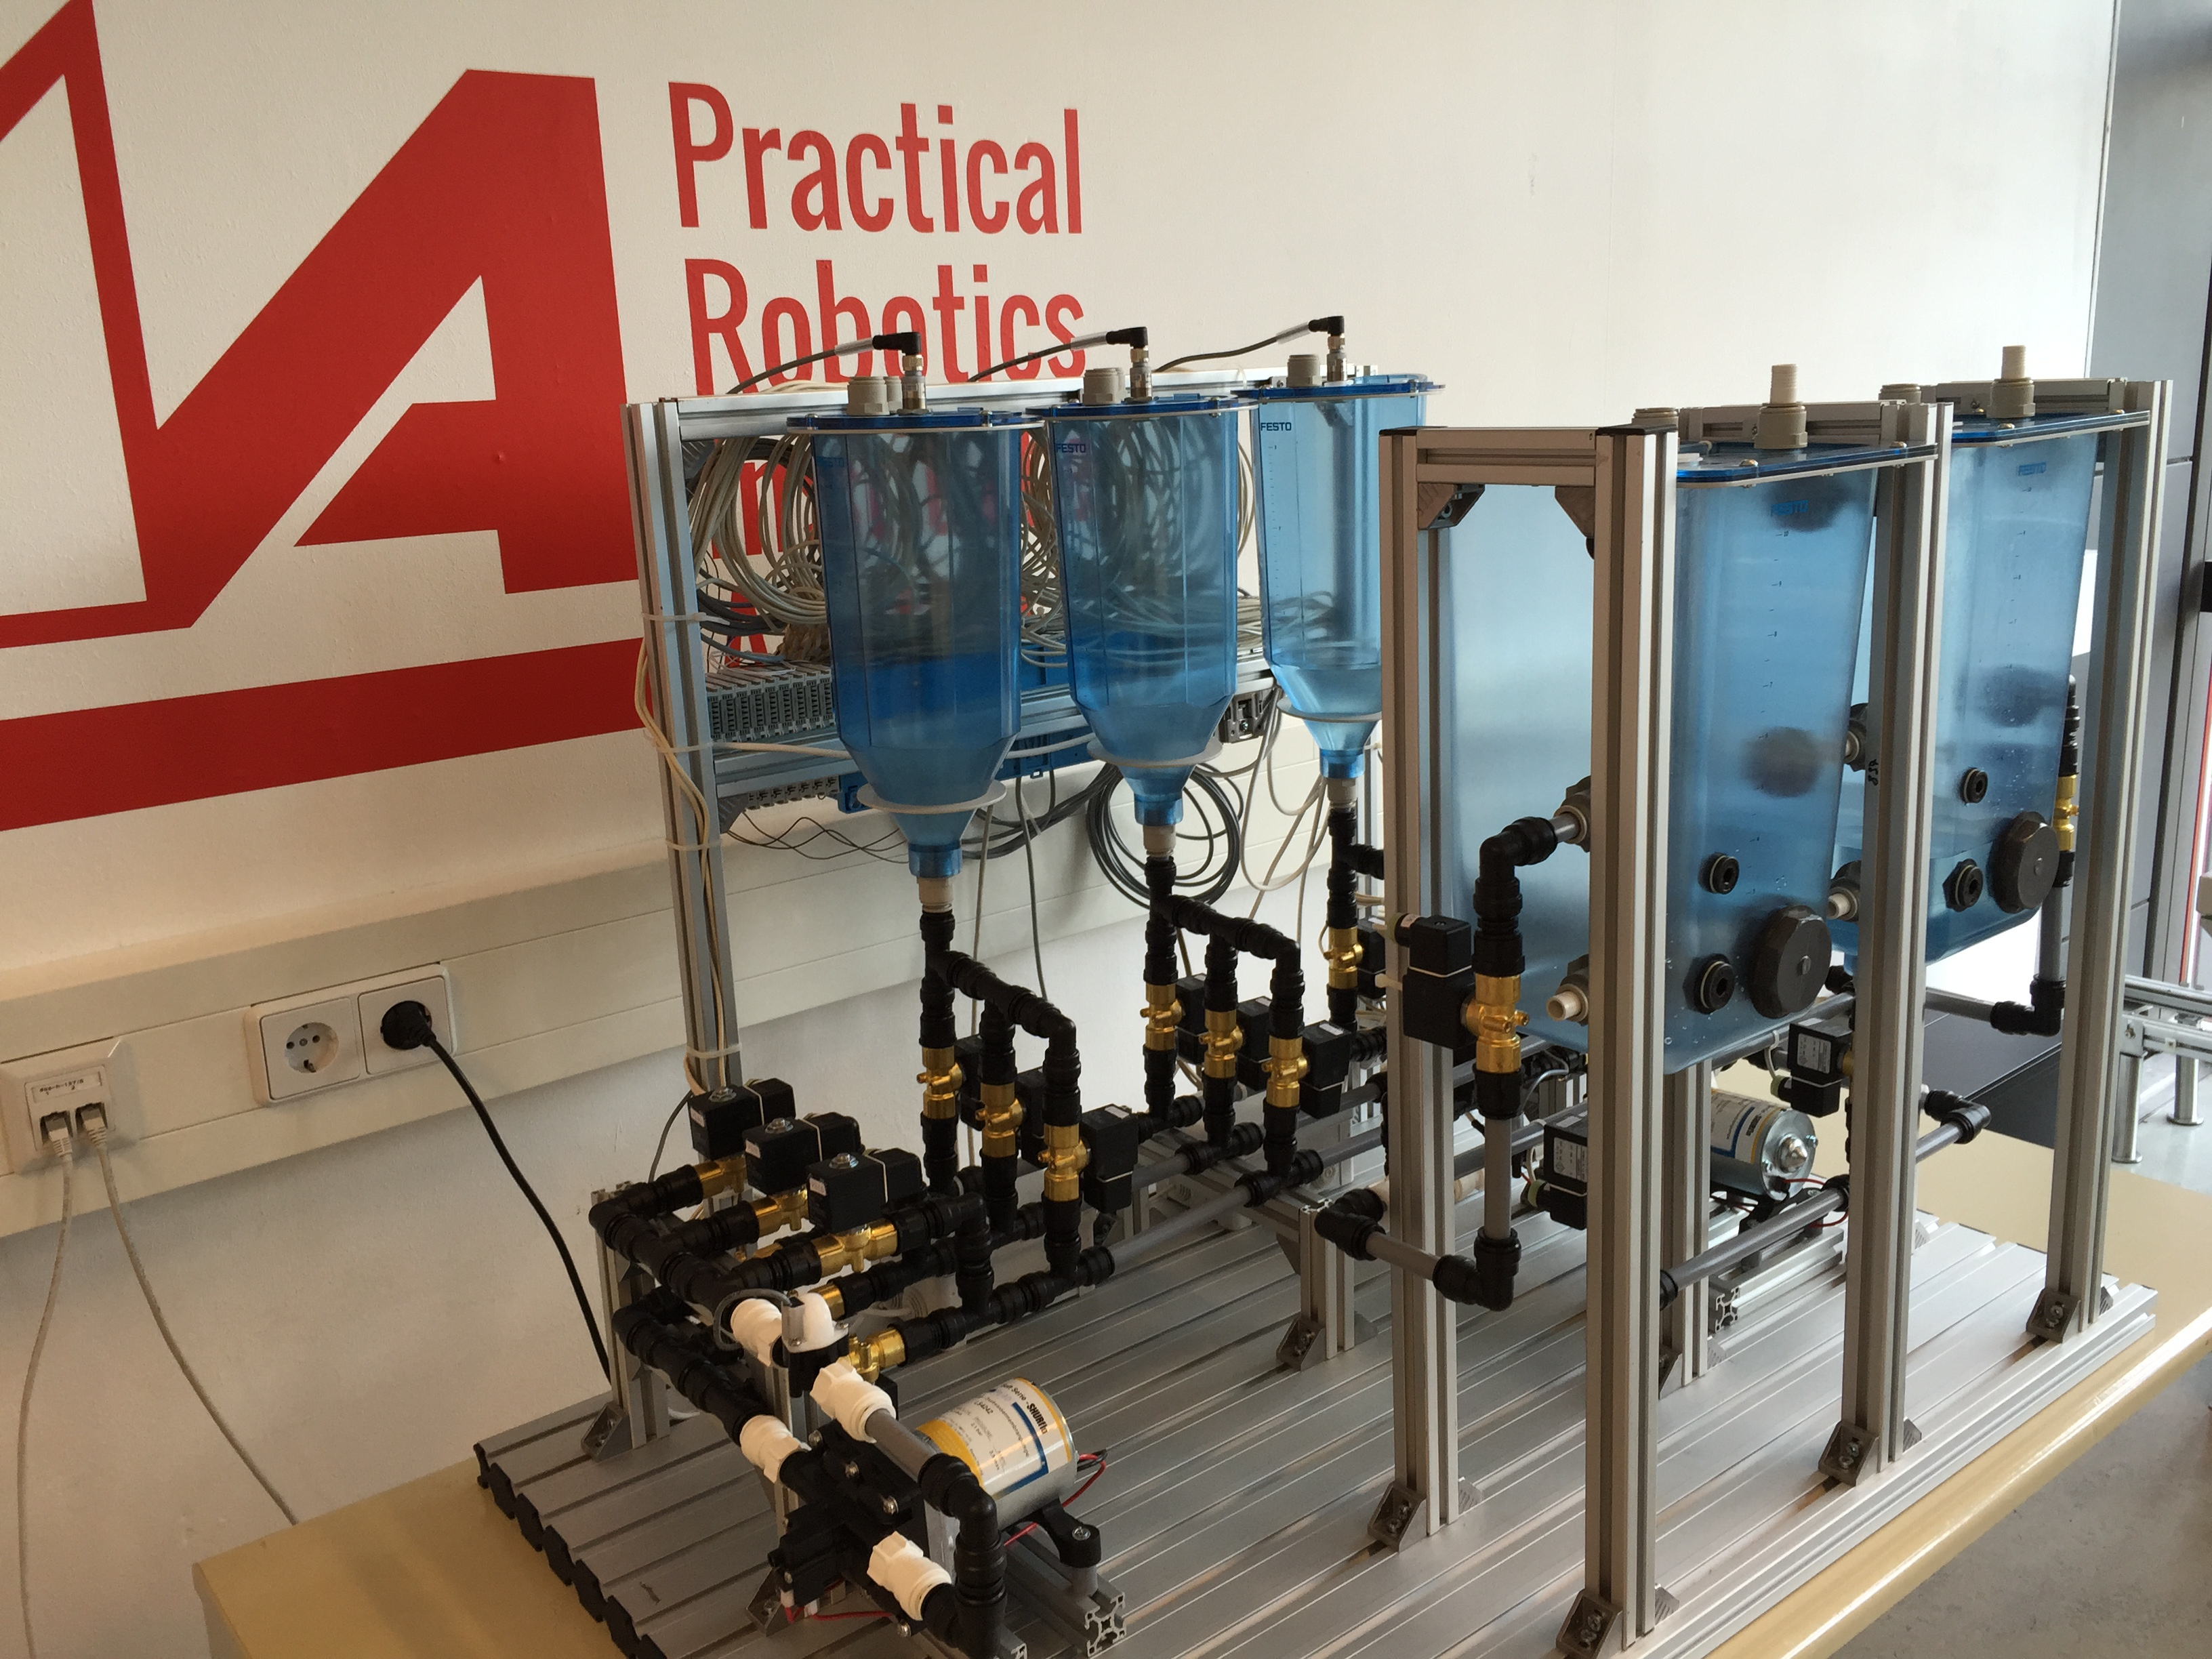
\includegraphics[width=0.8\textwidth]{graphics/implementation/FinalerAufbau.jpg}
	  \caption{Finaler Aufbau der Anlage}
	  \label{fig:finaler_aufbau}
	\end{figure}	

	\section{Prozeduren und Rezepte}
	Der Begriff Prozedur beschreibt das Zusammenfassen mehrerer Grundfunktionen einer Anlage, um einen Ablauf zu automatisieren. Zenon Batchcontrol, ein Unterprogramm der gewählten Softwarelösung, folgt der in IEC 61512 definierten Statemachine, einem von sich aus zustandswechselnden Automaten (siehe Abbildung~\ref{fig:statemachine}). Da eine \ac{SPS} dem zyklischen Abarbeiten programmierter Funktionen unterliegt, werden diese Zustände regelmäßig von Batch-Control an die Soft-\ac{SPS} Zenon Logic gesendet, die dann eine weitere Verarbeitung vornimmt und die angeforderte Statusänderung bestätigt. Durch global gesetzte Status kann so ein automatischer Wechsel der ausgeführten Funktionen erfolgen. Als Rezept wird das sequentielle Ausführen mehrerer Prozeduren bezeichnet, um einen weiteren Schritt der Automatisierung zu gehen.\\

\begin{figure}[h!]
  \centering
  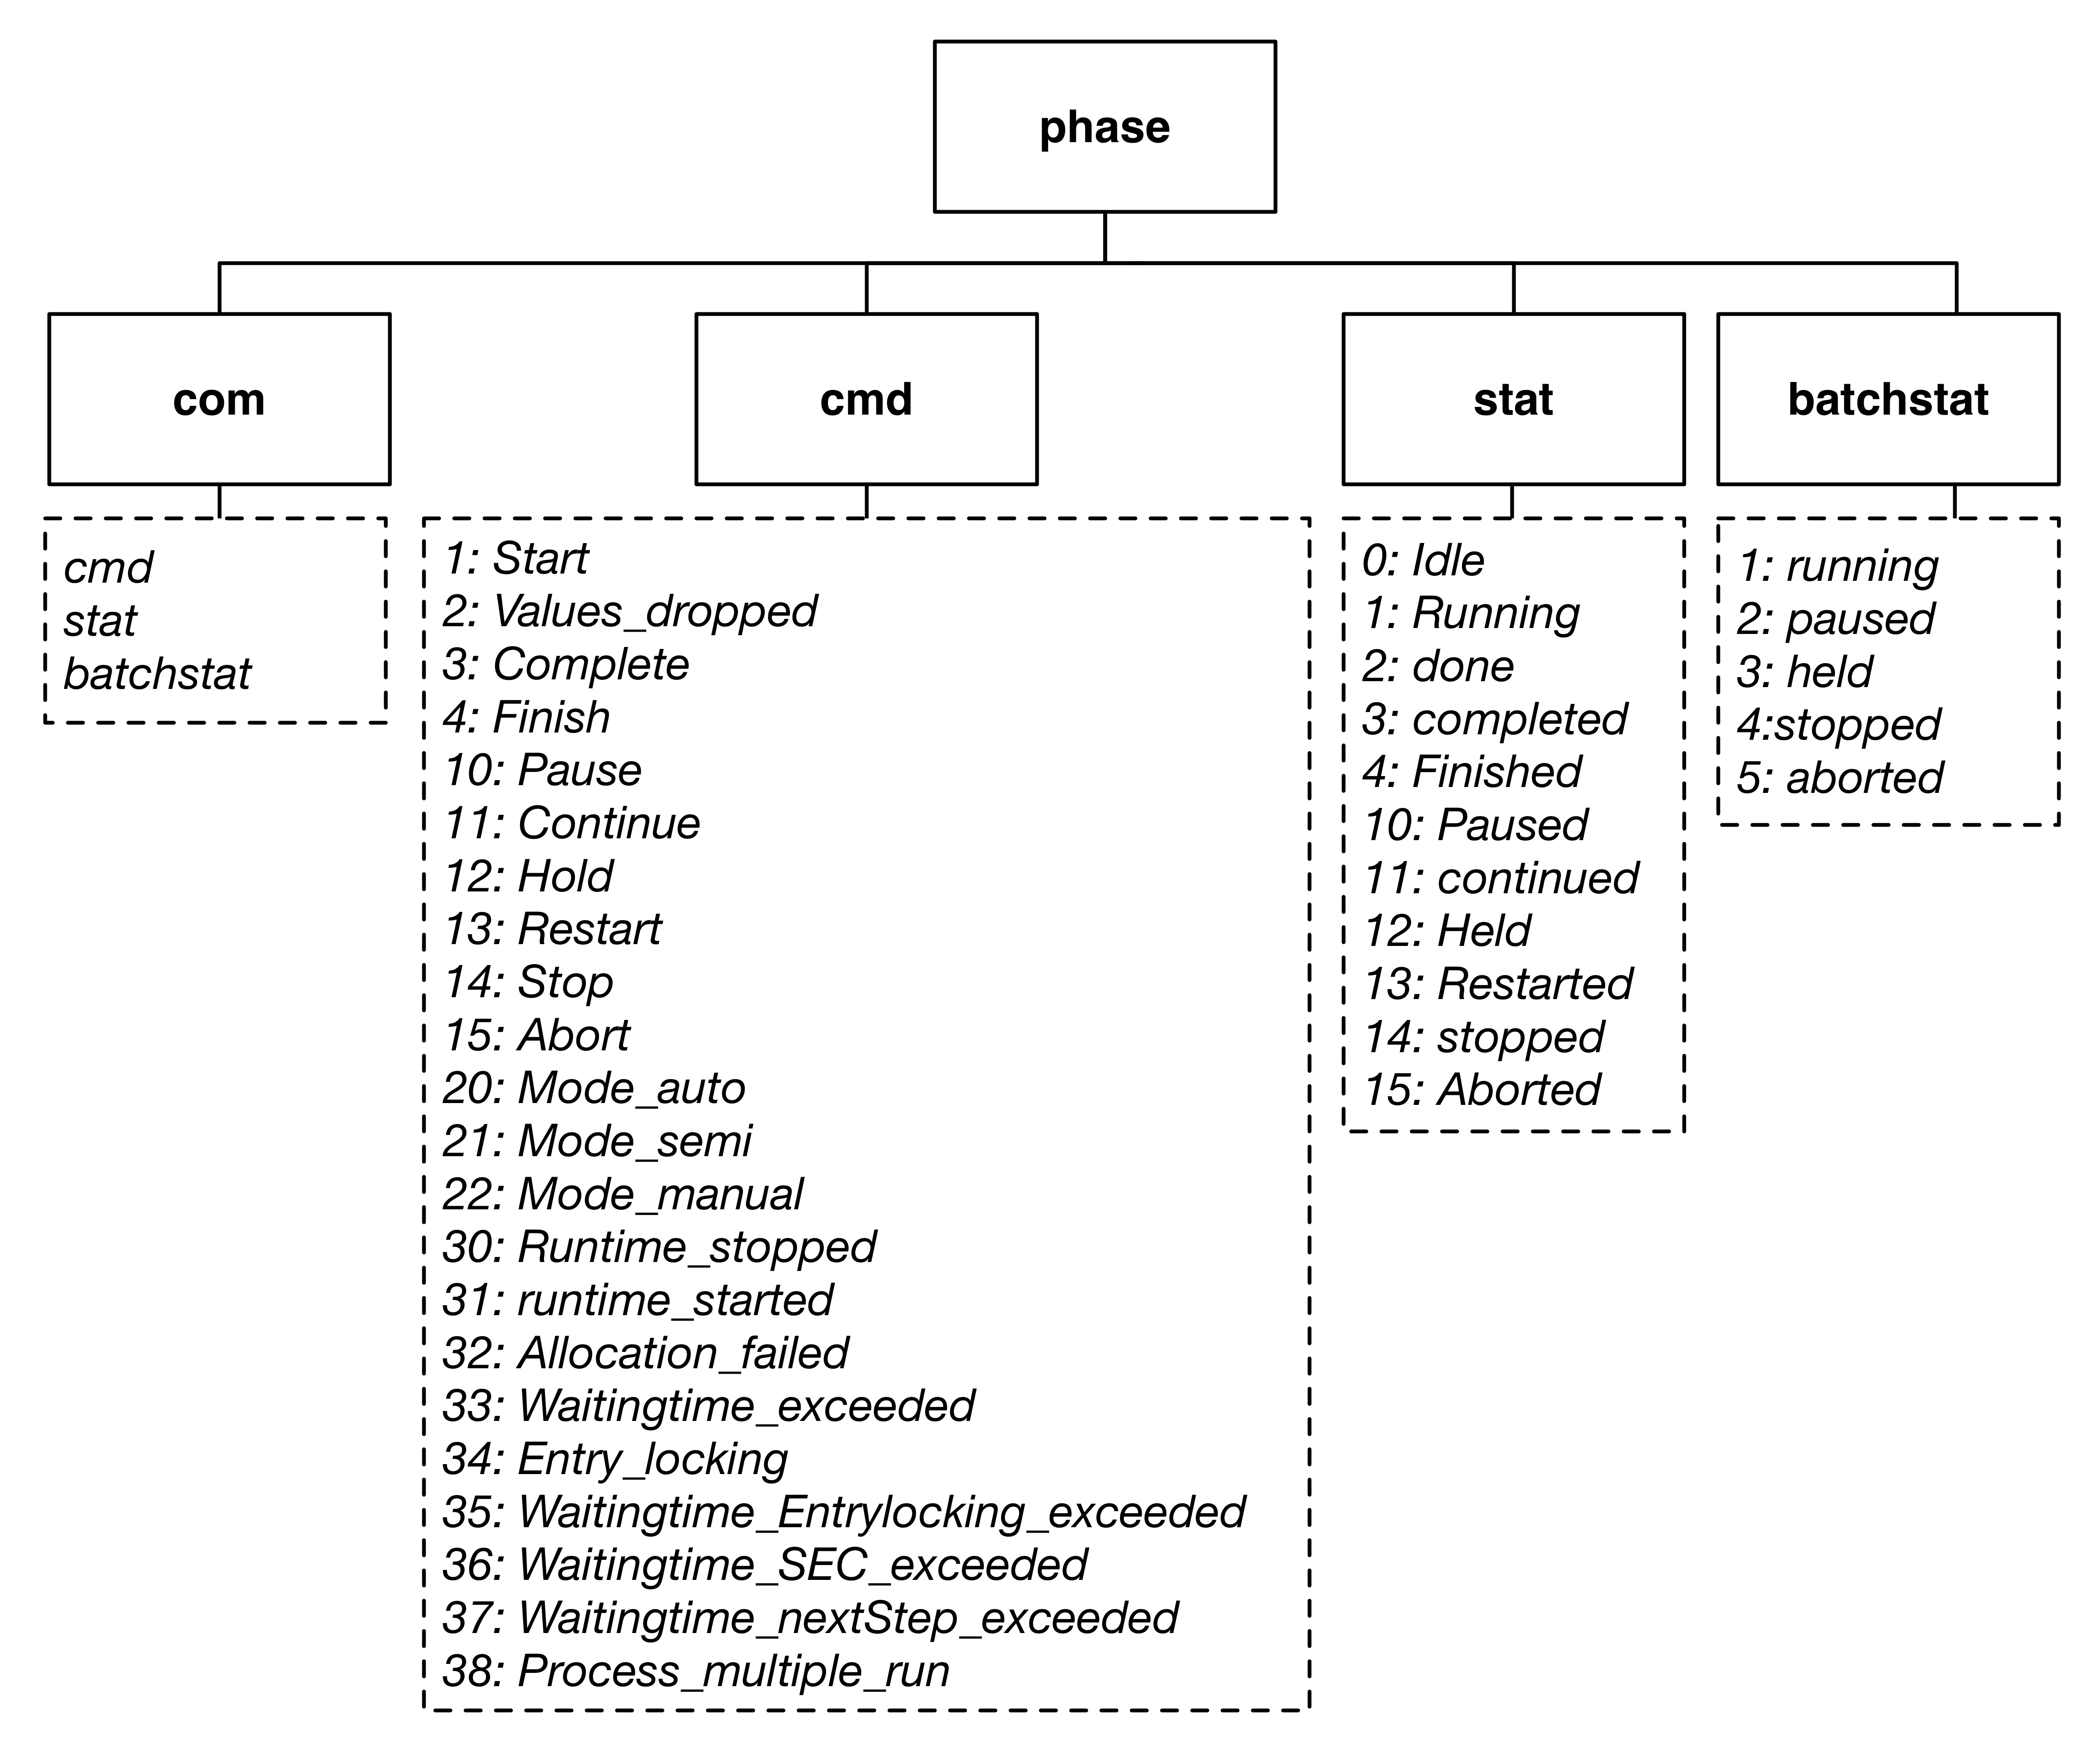
\includegraphics[height=0.6\textwidth]{graphics/implementation/Datentyp_Phase.jpg}
  \caption{Aufbau der Strukturvariable \glqq \textit{phase}\grqq}
  \label{fig:var_phase}
\end{figure}
	
	Für die Kommunikation zwischen einer Prozedur bzw. eines Rezepts und der \ac{SPS} stehen drei Kommunikationsvariablen (cmd, stat, batchstat) sowie eine weitere Strukturvariable (com) zur Verfügung (siehe Abbildung~\ref{fig:var_phase})
	
	\begin{itemize}
		\item Kommando: Sendet Befehle an \ac{SPS}-Grundfunktion
		\item Status: Empfängt internen Status der \ac{SPS}-Grundfunktion
		\item Batchstatus: Sendet internen Status des Rezepts zur \ac{SPS}
	\end{itemize}

	\textit{Kommando} trägt der \ac{SPS} auf, welcher Arbeitsschritte ausgeführt werden müssen. Mit dem \textit{Status} wird der Software zenon mitgeteilt, in welchem Stadium sich die Prozedur zum aktuellen Zeitpunkt befindet. Die Variable \textit{Batchstat} repräsentiert eine qualitätssichernde Redundanz, da der Status der \ac{SPS} teilweise in den Zustand 'running' wechselt, jedoch der interne Zustand von Batch Control diesen noch nicht erreicht hat. Zusätzlich erreicht in wenigen Fällen die \ac{SPS} den Status 'done', während Batch Control unterdessen noch nicht einmal den internen Zustand auf 'running' gesetzt hat. Mit Hilfe dieser zusätzlichen Variable kann die Prozedur nur dann auf 'done' schalten, wenn die \ac{SPS} \textbf{und} Batch Control den Zustand 'running' besitzen.\\
	
	Um eine Prozedur in zenon zu konfigurieren, benötigt es eine ganze Anzahl an zu erledigenden Arbeitsschritten. Initialisierend wird im Unterpunkt Batch Control ein neues Aggregat mit einer sich darin befindlichen neuen Grundfunktion (Prozedur) angelegt. Die Prozedur benötigt nun die zuvor erwähnten Kommunikationsvariablen Command, Status und Batchstatus. Zu beachten ist allerdings, dass es diese Strukturvariable bereits in der Form \glqq \textbf{name}.com.*\grqq \space geben muss, da andernfalls das Prinzip der Statemachine nicht eingehalten werden kann. Abermals untergeordnete Reaktionen werden mit den gewünschten Ereignissen befüllt, wobei wiederum zu beachten ist, dass diese den richtigen Variablen zugeordnet sind.\\

	Weitere Arbeitsschritte werden mittels Zenon Logic abgearbeitet. Ein Hauptprogramm, welches zum Ausführen aller anderen Funktionen dient, wird angelegt. Aufgerufene Unterprogramme sind \textit{get\_cmd()}, \textit{get\_batchstat()}, die auszuführende(n) Prozedure(n) und \textit{send\_state()}. Diese müssen vor dem ersten Durchlauf des Hauptprogramms angelegt sein.\\
	
	\subsection{get\_cmd()}
	Das Unterprogramm dient zum Null setzen (\glqq false\grqq \space setzen) aller Boolean-Werte die einen Status repräsentieren um alle gesetzten Werte zurückzusetzen. Desweiteren werden alle zur Auswahl stehenden Kommandos iteriert und nur die Variable des zutreffenden Kommandos gesetzt (\glqq true\grqq \space gesetzt).

	\lstinputlisting[caption=get\_cmd(),style=ST]{extra/get_cmd.txt}

	\subsection{get\_batchstat()}
	Dieses Unterprogramm setzt den zutreffenden aktuellen Status der Grundfunktion.
	
	\lstinputlisting[caption=get\_batchstat(),style=ST]{extra/get_batchstat.txt}

	\subsection{Prozedur}
	Innerhalb dieses Unterprogramms werden die Variablen bis zur Abbruchbedingung gesetzt.
	
	\lstinputlisting[caption=Prozedur,style=ST]{extra/prozedur.txt}

	\subsection{send\_state()}
	Dieses Unterprogramm dient zum globalen Setzen des aktuellen Status.
	
	\lstinputlisting[caption=send\_status(),style=ST]{extra/send_status.txt}
		
\begin{figure}[h!]
  \centering
  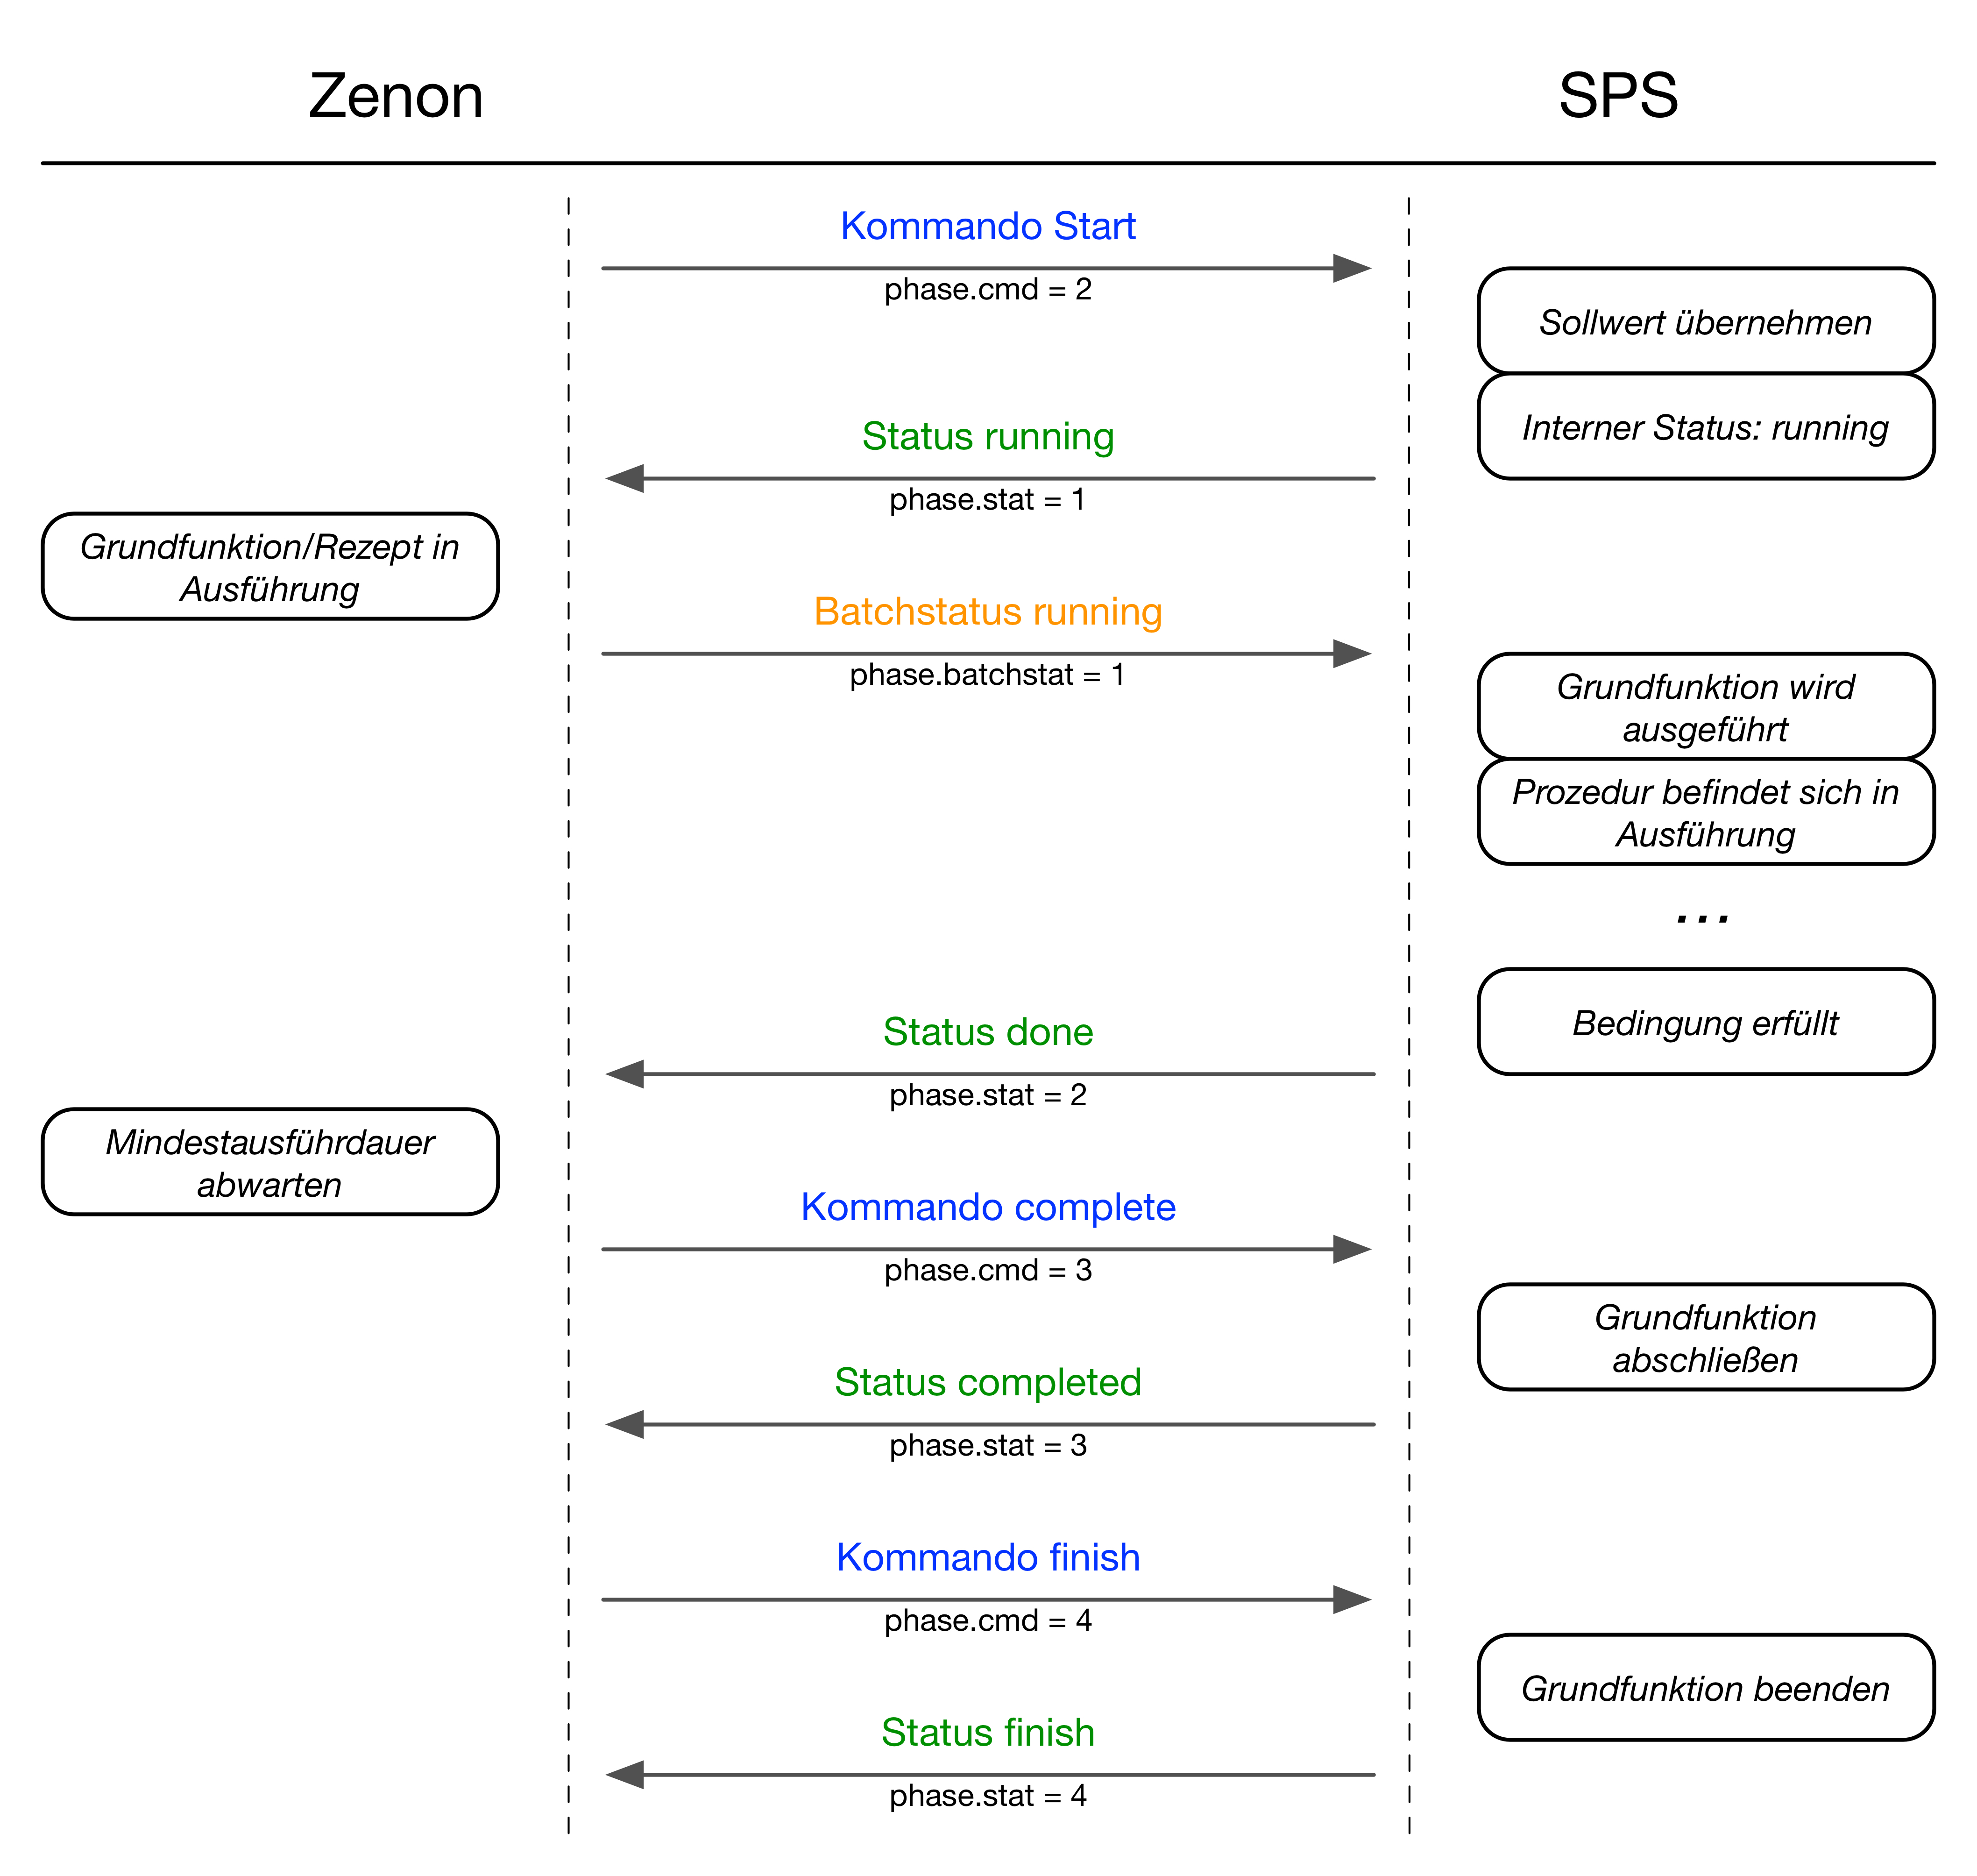
\includegraphics[width=1\textwidth]{graphics/implementation/StateMachine.jpg}
  \caption{Kommunikationsmodell von zenon und \ac{SPS} \space \cite{demo_zenonbatch}}
  \label{fig:statemachine}
\end{figure}

	Die Prozedur benötigt als zu setzenden Eingangsparameter die vorhandene Strukturvariable \glqq phase\grqq \space vom Typ \textit{phase}. Abschließend, vor Inbetriebnahme der Prozedur muss eine Weiterschaltbedingung definiert werden. Dazu wird im Unterpunkt Batch Control in den Eigenschaften der Grundfunktion der Menüpunkt Allgemein ausgewählt und die Weiterschaltbedingung eingefügt. Diese gilt für alle angelegten Grundfunktionen, da es sich dabei lediglich um das vergleichen der Status der Software zenon und \ac{SPS} handelt.

\lstinputlisting[caption=Beispiel einer Weiterschaltbedingung,style=ST]{extra/weiterschaltbedingung.txt}
	
	Zusätzlich werden wiederum zwei weitere Parameter (Status, Command) zum Weiterschalten benötigt. (siehe Abbildung~\ref{fig:weiterschaltbedingung})\\
	
\begin{figure}[h!]
  \centering
  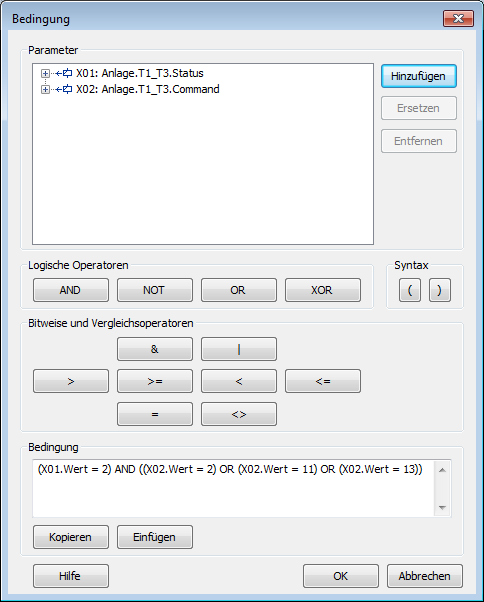
\includegraphics[height=0.8\textwidth]{graphics/implementation/weiterschaltbedingung}
  \caption{Weiterschaltbedingung einer Prozedur}
  \label{fig:weiterschaltbedingung}
\end{figure}

Zum jetzigen Zeitpunkt sind alle relevanten Komponenten einer Prozedur erstellt worden. In der Oberfläche kann nun anschließend mittels einer definierten Eingabeoberfläche eine Prozedur oder ein vollständiges Rezept erzeugt werden. Zusätzlich ist es möglich, Grundfunktionen oder Rezepte zu pausieren, im Nachhinein zu editieren oder zu stoppen. Zusammengefasste Grundfunktionen (Rezepte) können weiteres in der erstellten Form inklusive zusätzlicher Informationen abgespeichert werden.

\begin{figure}[h!]
  \centering
  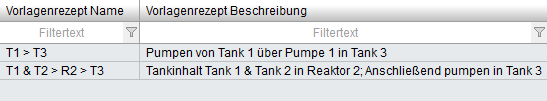
\includegraphics[width=1\textwidth]{graphics/implementation/rezepte_liste}
  \caption{Liste der gespeicherten Rezepte}
  \label{fig:rezepte_list}
\end{figure}
	
\section{\ac{HMI}}
Für dieses Projekt wurde als SCADA System die Software zenon vorgegeben, daher wird das \ac{HMI} in zenon Supervisor (zenons \ac{HMI} Programm) umgesetzt.\\
\\
\textbf{Visualisierung}\\
In zenon wird eine Visualisierung \glqq Bild\grqq\space  gennant. Dieses kann mit vorgefertigten Elementen erweitert werden. 

Als Ausgangspunkt für die Visualisierung wurde das \ac{RI} zur Hand genommen. Aus diesem wurde die Anzahl der Elemente und die Grundstruktur übernommen. Als nächsten Schritt musste evaluiert werden, welche Inhalte des \ac{RI} für die Visualisierung relevant und welche Informationen nicht vorhanden waren.\\
\begin{figure}[hbt!]
  \centering
  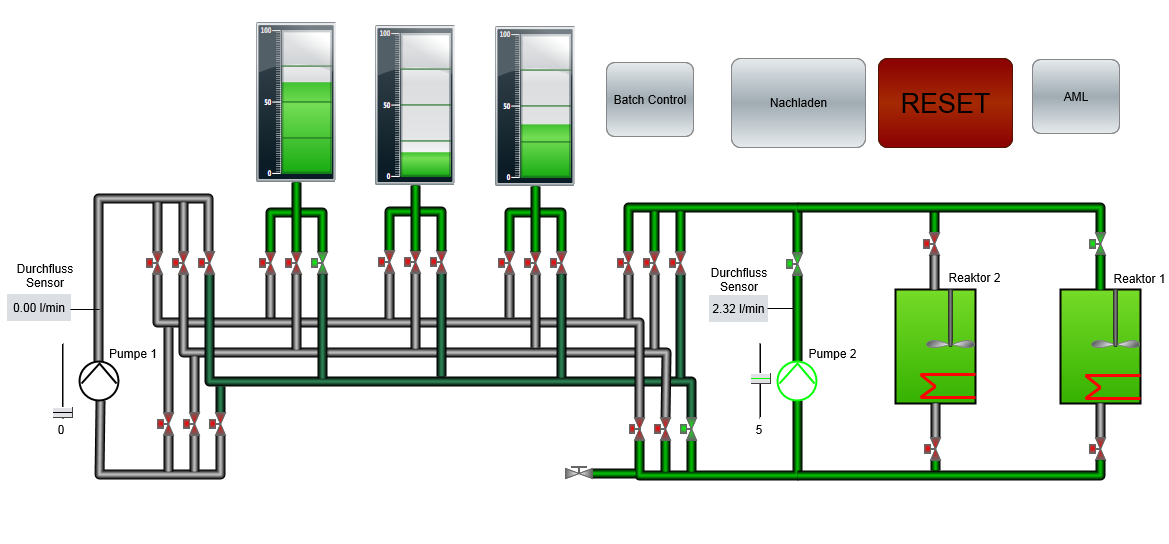
\includegraphics[width=1\textwidth]{graphics/implementation/Visualisierung}
  \caption{Umsetzung der Visualisierung in zenon}
\end{figure}
\\
\newpage
\textbf{Feldbuskonfiguration}\\
Um eine Visualisierung mit aktuellen Sensorwerten zu befüllen, wird eine Verbindung zur \ac{SPS} benötigt. Diese Verbindung wird über das Teilprogramm zenon Logic (im weiteren nur noch Logic genannt) hergestellt.\\
\\
Als ersten Schritt, um in Logic eine \ac{SPS} hinzuzufügen, muss im Unterpunkt \glqq Feldbuskonfiguration\grqq\space die Treibersoftware für die ADAM5550 \ac{SPS} hinzugefügt werden. Daraufhin müssen alle Module, die an der \ac{SPS} angebracht sind, in die Konfiguration hinzugefügt werden.\\
\begin{figure}[h!]
  \centering
  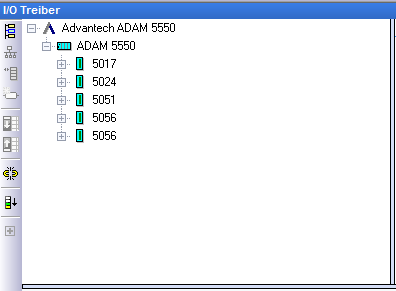
\includegraphics[width=0.7\textwidth]{graphics/implementation/Feldbuskonfiguration}
  \caption{Feldbuskonfiguration für eine \ac{SPS} in zenon}
\end{figure}
\\
\textbf{Variablen}\\
In zenon können auf mehrere Arten Variablen erstellt werden. Damit diese für die Visualisierung und von Logic sichtbar sind, müssen sie als Globale Variable definiert werden. Der einfachste Weg dafür ist es, im Logic Variablenfenster, über den Reiter  \glqq Globale Variablen\grqq, die Funktion \glqq Variable hinzufügen\grqq\space aufzurufen.\\
\\
Sobald alle Variablen erstellt sind, werden diese mit der Feldbuskonfiguration verknüpft. Durch diesen Schritt erhält man Zugang zu den an der \ac{SPS} angeschlossenen Bauteilen.

\newpage
\begin{figure}[h!]
  \centering
  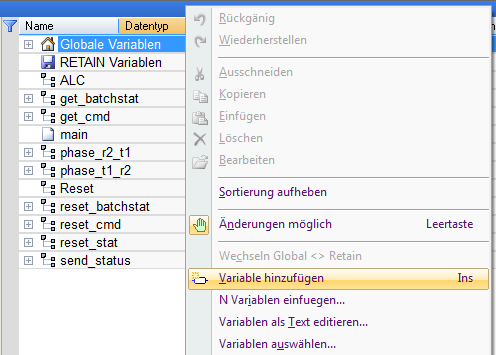
\includegraphics[width=0.7\textwidth]{graphics/implementation/Variablen}
  \caption{Variablen erstellen in zenon Logic}
\end{figure}

\textbf{Steuerung}\\
\\
Phase 1 Steuerung mittels Buttons:\\
	Der erste Versuch war es die Steuerung mittels einfachen Buttons umzusetzen. Diese haben meist die in zenon vorhandene Funktion  \glqq Sollwert absetzen\grqq\space  verwendet, welche den Wert einer Variable ändert.\\
	So konnten alle Funktionen umgesetzt werden, dadurch erhielt das  \glqq Bild\grqq\space  jedoch viele Elemente die von der Eigentlichen Visualisierung ablenkten.\\
\\
Phase 2 Versteckte Buttons:\\
	Um den Element-Overload zu verringern war der nächste Schritt die Buttons zu  \glqq verstecken\grqq\space  indem sie Transparent über die eigentlichen Elementen (beispielsweise ein Ventil) verschoben wurden.\\
	In der Visualisierung wurden nun weniger  \glqq unwichtige\grqq\space  Bausteine angezeigt, die Elemente waren jedoch immer noch da, wodurch die Speichergröße der Visualisierung deutlich anstieg.\\
\\
Phase 3 Funktionale Elemente:\\
	Der nächste schritt war es die nicht funktionalen Grafikelemente durch Buttons in Form der gewünschten Elemente zu ersetzten.\\
\\

\section{Ontologie}
Nachdem die Evaluierung der wichtigsten Aspekte im Kapitel Ontologie der Chargenprozessanlage in Hinsicht auf eine automatisierte Codegenerierung durchgeführt wurden, behandelt dieses Kapitel den Werdegang der Ontologie vom Ersten bis hin zum finalem Design.\\
\\
Das Ziel der Ontologie ist es, die im laufe dieses Projekts aufgebaute Anlage in einer Art und Weise abbilden zu können, die es erlaubt daraus eine automatisierte Codegenerierung durchzuführen und dabei auf einem Abstraktionslevel zu bleiben um einen Großteil an in der Industrie vorkommenden Produktionsanlagen abbilden zu können.\\
\\
Da es den Rahmen dieser Arbeit sprengen würde, auf jeden einzelnen Gedankengang in der Erstellung der Ontologie einzugehen, werden nur die großen Revisionen der Ontologie genauer beschrieben.\\
\\
Zu Beginn werden alle Bauteile der Anlage in Kategorien eingeteilt. Tanks, Reaktoren und Pumpen sind die Hauptelemente der Anlage und werden deswegen auch in einer Gruppe zusammengefasst. Neben ihnen gibt es eine Gruppe an Bauteilen die steuerbar sind, hierzu gehören die Ventile, Sensoren, Heiz- und Rührstäbe. Die restlichen Elemente der Anlage sind statische Objekte die einen Nutzen haben, jedoch keine Arbeit erledigen. Daher fallen diese zusammen unter die Kategorie von passiven Elementen. Zu diesem Zeitpunkt sind das nur die Rohre.\\

Eine Ausnahme dieser Gruppen ist die \ac{SPS}, welche steuerbar ist und daher in Kategorie 2 fallen würde. Da sie aber nicht direkt Teil der Anlage ist, findet sie einen Platz als einzelstehendes Objekt in der Ontologie. Verbindungen zwischen zwei Klassen werden normalerweise mit einer Objekt Eigenschaft dargestellt. Da eine Verbindung zwischen zwei Bauteilen mehr Informationen als die Verbindung zwischen einer \ac{SPS} und einem Bauteil enthält, gibt es die Kategorie Connections mit den Klassen “Weg” und “IO”. \\

Kurz zusammengefasst können die Kategorien wie folgt beschreiben werden\\

\begin{figure}[hbt!]
  \centering
  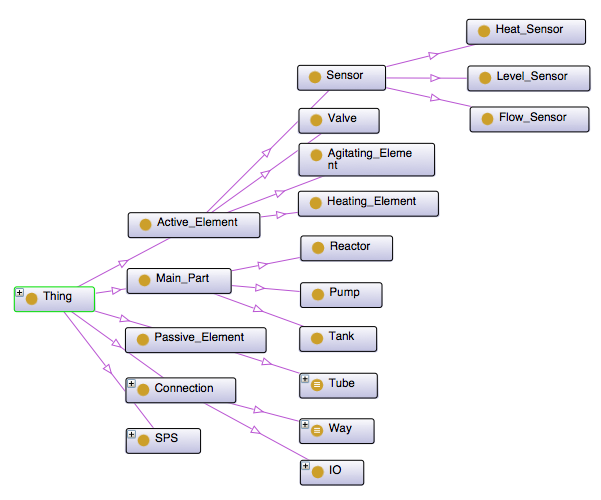
\includegraphics[width=0.7\textwidth]{graphics/implementation/Ontology_v1}
  \caption{Erste Version der Ontologie}
\end{figure}

\textbf{Main\_Part:}\\
	Alle Elemente die subjektiv als Hauptelemente bezeichnet werden können.\\

\textbf{Active\_Element:}\\
	Jene Bauteile die steuerbar sind. (Aktuatoren, Sensoren)\\

\textbf{Passive\_Elements:}\\
	In der Anlage verbaute Teile, die keine Arbeit verrichten.\\ 

\textbf{Connection:}\\
	Verbindungsarten zwischen den einzelnen Bauteilen.\\
\\
Mit dieser Ontologie ist es grundsätzlich möglich die Anlage aus Kapitel 4.2 abzubilden, jedoch finden sich einige Inkonsistenzen, die die automatisierte Codegenerierung erschweren wenn nicht sogar unmöglich machen würden.\\

Ein Beispiel dafür wäre die Pumpe, welche bei \glqq Main\_Part \grqq\space untergebracht ist. Jedoch wurde die Gruppe der \glqq Active\_Elements\grqq\space als Aktuatoren bestimmt. Dies hätte zur Folge, dass bei einer automatisierte Codegenerierung für Aktuatoren in verschiedenen Plätzen gesucht werden müsste.\\
\\
In Hinsicht einer automatisierten Codegenerierung wird die erste Version der Ontologie evaluiert und dementsprechend umgebaut.
Die Kategorien werden im nächsten Schritt genauer definiert um eine Konsistenz in die Ontologie zu bringen.\\
\\
Die Definition von \glqq Active\_Element\grqq\space ist im Grunde richtig, allerdings ist die SPS in \glqq Active\_Element\grqq\space beinhaltet. Daher wird die Definition auf \glqq Elemente die mit einer \ac{SPS} (I/O) verbunden sind\grqq\space geändert. In diese Kategorie fallen nun die Elemente der ersten Version ohne \ac{SPS} und Pumpe hinein.\\
\\
Die nächste Kategorie ist \glqq Main Part\grqq. Die Definition dieser Gruppe ist sehr grob definiert und lässt eine subjektive Gruppierung zu, daher muss die Definition von Grund auf geändert werden. Die passende Interpretation ist \glqq Elemente mit mindestens zwei Ein bzw. Ausgängen\grqq. Durch diese Änderung fallen nun auch die Ventile in die Gruppe \glqq Main Part\grqq.\\
\\
Um Ein-/Ausgänge besser zu definieren wird die Gruppe \glqq Connection\grqq\space verändert. Die Klasse \glqq I/O\grqq\space wird heraus genommen, da man diese genauer beschreiben muss. Dadurch enthält \glqq Connection\grqq\space nur noch Verbindungen zwischen Bauteilen, welche Ein-/Ausgänge sein können.\\
\\
Die Kategorie \glqq Passive Element\grqq\space wird komplett entfernt, da sie keine relevanten Information enthält.

\begin{figure}[hbt!]
  \centering
  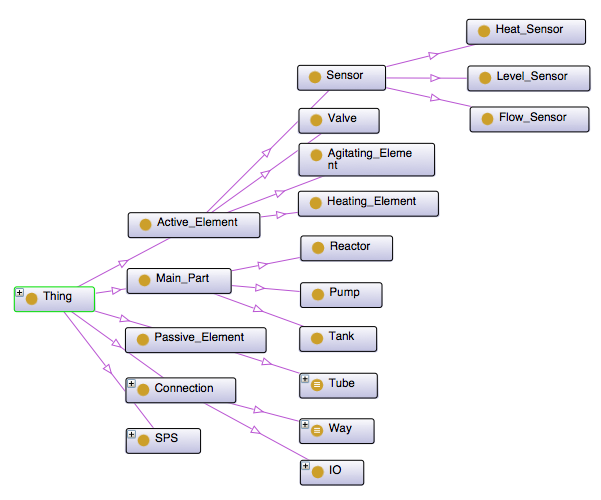
\includegraphics[width=0.7\textwidth]{graphics/implementation/Ontology_v2}
  \caption{Erste Überarbeitung der Ontologie}
  \label{fig:v2_ontology}
\end{figure}

Von diesem Punkt aus wird die Ontologie nur noch verfeinert und nicht mehr großartig an der Struktur gearbeitet.
Die Klasse \ac{SPS} wird, um Konsistenz in die Namen zu bringen, in die englische Bezeichnung \ac{PLC} umbenannt. \\\\ 
Die Änderungen, die von Abbildung \ref{fig:v2_ontology} hin zur finalen Version der Ontologie Abbildung \ref{fig:final_ontology} gemacht wurden, sind trivial. Dazu gehört das Entfernen der Subklasse \glqq Sensoren\grqq, um den Aufwand für die Codegenerierung zu verringern.\\

\begin{figure}[hbt!]
  \centering
  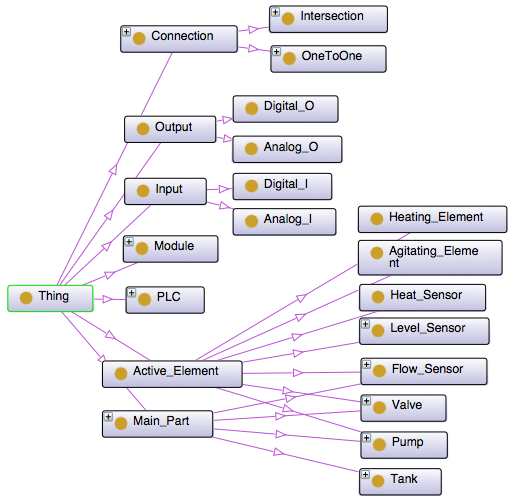
\includegraphics[width=0.7\textwidth]{graphics/implementation/Ontology_final}
  \caption{Finale Version der Ontologie}
  \label{fig:final_ontology}
\end{figure}
\begin{table}[h]
\centering
\begin{tabular}{l|l|l}
\textbf{Name} & \textbf{Domain} & \textbf{Range} \\ \hline
hasActiveE    & Input, Output   & Active\_Element \\ \hline
hasConnection & MainPart        & Connection      \\ \hline
hasIO         & Module          & Input, Output   \\ \hline
hasModule     & PLC             & Module          \\ \hline
isIncludedTo  & Tank            & Active\_Element \\ \hline
isConnectedTo & Connection      & Connection                            
\end{tabular}
\end{table}
\newpage
\textbf{Object Properties}\\
Nachdem die Klassenstruktur feststeht, müssen als nächstes die Relationen bestimmt werden. Mit Hilfe von Object Properties lassen sich alle Verbindungen zwischen den jeweiligen Elementen/Klassen abbilden.\\
\\
\textbf{Data Properties}\\
Die Ontologie besteht nun aus Klassen und deren Relationen, jetzt muss sie mit Eigenschaften erweitert werden, um eine Codegenerierung zu ermöglichen.
Dafür wurden die folgenden Data Properties erstellt:\\\\
\textbf{capacity: }Das Volumen bzw. die Füllmenge eines Tanks. Der Datentyp ist ein Integer.\\

\textbf{direction: }Gibt die Richtung einer Connection an.\\

\textbf{maximum: }Der maximaler Wert mit dem das Element angesprochen werden kann, bzw. maximal Wert den das Element zurück liefert.\\

\textbf{minimum: }Der kleinster Wert mit dem das Element angesprochen werden kann, bzw. minimal Wert den das Element zurück liefert.\\

\textbf{offstate: }Signal bei dem das Element stoppt bzw. schließt.\\

\textbf{signal: }Dies ist ein numerischer Wert, der entweder eins oder zwei sein kann. Eins steht dafür, dass das Element digital ist. Zwei steht dafür, dass das Element analog ist.\\

\section{Aktivitätsdiagramm}

Im vorigen Kapitel wurde der Werdegang der Ontologie genauer beschrieben. Um auch Prozeduren automatisch generieren zu lassen, wird ein Diagramm bzw. eine Aufzählung von den gewollten Prozeduren benötigt.\\
Im Gegensatz zu der Erstellung der Ontologie ist das Design bzw. der Aufbau dieses Diagramms schon vor der ersten Iteration klar definiert.\\
\\
In diesem Projekt wird eine sehr vereinfachte Form eines Aktivitätsdiagramms verwendet, da mit diesen Diagrammen die benötigten Informationen (Namen, Abbruchbedingungen, etc.) übermittelt werden können.\\

\begin{figure}[hbt!]
  \centering
  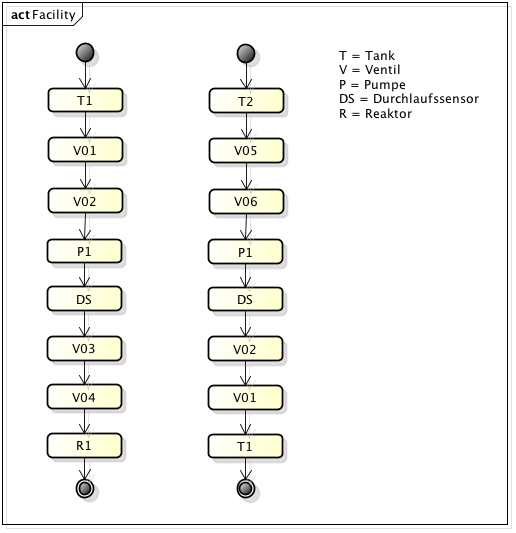
\includegraphics[width=0.7\textwidth]{graphics/konzept/UML_Activity}
  \caption{Diagramm für zwei Prozeduren}
\end{figure}
Die wirkliche Aufgabe bei diesem Diagramm ist es herauszufinden, welche Daten man zu den jeweiligen Elementen hinzufügen muss, um eine Codegenerierung bestmöglich durchführen zu können.\\
Dies ist ein langwieriger Prozess der bis zur Fertigstellung der Codegenerierung andauert, da erst beim automatischem Erstellen der Prozeduren klar wird, welche Informationen hinzugefügt werden können um das Ergebnis der Codegenerierung zu verbessern.\\
\\
Um den generierten Prozeduren einen Namen geben zu können, befindet sich im Startknoten das Attribut \glqq name\grqq. Neben diesem befindet sich noch ein weiteres \glqq verstecktes Attribut\grqq, dass die Abbruchbedingung der jeweiligen Prozedur angibt.\\

In den einzelnen Zuständen der Aktivität, die jeweils ein Element der Anlage abbilden, befindet sich ein Attribut mit dem Wert, der in der Prozedur für diesen Schritt benötigt wird. Beispielsweise bei den Ventilen (V1,V2,...) der Wert \glqq 1\grqq\space und bei der Pumpe ein Mittelwert, der nach der Generierung vom Benutzer genauer definiert werden kann. Abgeschlossen werden alle Prozeduren in dem Diagramm mit einem Endknoten, wie es in einem vollständigen Aktivitätsdiagramm der Fall ist.\\
\newpage
\section{Codegenerierung}

Die Codegenerierung könnte in unterschiedlichsten Sprachen erfolgen, jedoch können nur über Zenon Wizards auch direkte Eingriffe auf ein Zenon Projekt vorgenommen werden. Es gibt zwei Arten von Zenon Wizards, die sich durch die Benutzeroberfläche unterscheiden, aber auch mit verschiedenen in zenon integrierten Editoren erstellt werden. Die Editoren untersützen außerdem unterschiedliche Sprachen. Die verfügbaren Editoren sind \ac{VSTA} und \ac{VBA}.\\
Es wird \ac{VSTA} verwendet, da hier die grafische Benutzeroberfläche ansprechender ist. Die Funktionalität mit \ac{VBA} deckt sich größtenteils.\\

Der erste wichtige Punkt ist es herauszufinden, wie weit die Prozeduren und Rezepte automatisiert werden können. Hierfür wird die zenOn Library in \ac{VSTA} verwendet, die schon integriert ist. \ac{VSTA} unterstützt mehrere Programmiersprachen, der Wizard wird jedoch in C\# geschrieben, da in C\# eine gute Unterstützung für \ac{XML} gegeben ist.

\subsection{Datentyp anlegen}
Um ein Element der Anlage im Programm abzubilden, werden einige Attribute benötigt, weshalb hier ein Strukturdatentyp erstellt wird. Dieser wird den Namen des Elements erhalten und alle in der Ontologie abgebildeten Attribute beinhalten.

\lstinputlisting[caption=Anlegen eines Datentyps in zenon,style=csharp]{extra/createdatatype.txt}
\newpage
\subsection{Variable anlegen}
Damit der aktuelle Zustand, sowie die weiteren Attribute jedes eingebauten Elements der Anlage, abgespeichert werden können, muss für eben jedes dieser eine eigene Variable angelegt werden. Eine Variable muss an einen Treiber angebunden werden, wobei die Auswahl durch den Benutzer über die Benutzerschnittstelle erfolgt. Damit die Variable global, also auch in Zenon Logic, erreichbar ist, muss sie in einem Namespace sein. Dies wird dadurch erreicht, dass vor dem Namen der Variable ein „Logic/Global/“ hinzugefügt wird, wobei Logic hier der Name des Zenon Logic Projekts ist. Da alle durch die Codegenerierung angelegten Variablen verwendet werden um Teile unserer \ac{SPS} anzusprechen, muss als Kanal der „SPSMerker“ angeben werden.
\begin{figure}[hbt!]
  \centering
  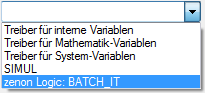
\includegraphics[width=0.4\textwidth]{graphics/implementation/treiberauswahl}
  \caption{Auswahl des zenon Logic Treibers}
\end{figure}

\lstinputlisting[caption=Anlegen einer Variable in zenon,style=csharp]{extra/createvar.txt}

\subsection{Ontologie als \ac{XML}}
Die Ontologie wird als \ac{XML} exportiert. Diese \ac{XML} Datei ist auf den Standards \ac{OWL} und \ac{RDF} aufgebaut, welche die Struktur und Aufteilung der abgebildeten Elemente vorgeben.\\

\textbf{\ac{OWL}:}, \textbf{\ac{RDF}:}, \textbf{rdfs:} sowie \textbf{Facility:} und \textbf{\&Facility;} sind Namespaces, also für den Namen selber nicht relevant, sie grenzen nur den Gültigkeitsbereich der Namen ab.\\
\newpage
Wichtig für die Codegenerierung sind folgende Tags:\\

\textbf{DatatypeProperty}\\
Dieser Tag enthält Informationen über ein Attribut. Die Informationen, die man entnehmen kann beinhalten den Namen und Datentyp des Attributs, sowie für welche Elemente sie anwendbar sind.\\
\lstinputlisting[caption=XML Struktur des DatatypeProperty Tags,label=lst:dtprop,style=XML]{extra/datatypeproperty.xml}
\textbf{Class}\\
Eine „Class“ entspricht einem Element, das in der Ontologie abgebildet ist. Es wird der Name angegeben und die Klassen, von welchen es erbt, also die Klassen deren Attribute es übernimmt.\\
\lstinputlisting[caption=XML Struktur des Class Tags,label=lst:class,style=XML]{extra/class.xml}

\textbf{NamedIndividual}\\
Das „NamedIndividual“ ist ein konkretes eingebautes Element der Anlage. Dieses hat einen Namen und Attribute mit zugewiesenen Werten.\\
\lstinputlisting[caption=XML Struktur des NamedIndividual Tags,label=lst:indiv,style=XML]{extra/namedindividual.xml}

\subsection{Generierung der Datentypen}
Die Datentypen entsprechen den Klassen in \ac{OWL}, sie bilden eine Objektstruktur durch die eine Variable dieses Typs angelegt werden kann. Zusätzlich zu den Klassen werden auch die in \ac{OWL} Datatype Properties genannten Ressourcen eingebracht werden, da diese die erforderliche Objektstruktur mit Subtypen genauer definieren.\\

Um dies zu erreichen, werden erst alle Datatype Properties aus der Ontologie ausgelesen und dessen Name, wie auch Datentyp, mit der zugehörigen Klasse verbunden. Als Beispiel in Listing \ref{lst:dtprop} ist z.B. das Attribut \textbf{offstate} mit dem Datentyp \textbf{int} (für ganzzahlige Werte) für alle Elemente der Klasse \textbf{Active\_Element} ersichtlich.\\

Da nach diesem Schritt alle Attribute verfügbar sind, können nun die Klassen angelegt werden. Um dies zu erreichen liest man alle Klassen aus der Ontologie aus und legt einen Datentyp für diese an. Listing \ref{lst:class} zeigt, dass das Element \textbf{Valve} eine Subklasse von \textbf{Active\_Element} ist, daher übernimmt es das Attribut \textbf{offstate} jedoch auch alle Attribute, die für \textbf{Valve} und \textbf{Main\_Part} registriert sind. Außerdem muss überprüft werden, ob das Element ein Main\_Part oder Active\_Element ist, da diese in der Ontologie als jene definiert sind, die über die Steuerung angesprochen werden können. Jedes Element bekommt zusätzlich noch das Attribut \textbf{value}, welches den aktuellen Wert anzeigen soll oder mit dem man den gewünschten Wert setzen kann.

\subsection{Generierung der Variablen}
Die für die Variablen wichtigen Elemente werden in \ac{OWL} als Named Individual abgebildet, welche also ausgelesen werden müssen um die Variablen anlegen zu können. Eine Voraussetzung um die Variablen anlegen zu können ist auch, dass die Datentypen bereits generiert wurden. In Listing \ref{lst:indiv} erkennt man, dass die Variable \textbf{V123} in mit drei Klassen in Verbindung steht: Valve, Main\_Part und Active\_Element). Also muss man um den Datentyp herauszufinden die Vererbungsstruktur dieser untersuchen, um das spezifischste zu finden. Durch die in Listing \ref{lst:class} ersichtliche Struktur der Klasse Valve kann man darauf schließen, dass Valve von Main\_Part und Active\_Element erbt, also ist dies die spezifischste Klasse. Das Named Individual enthält zusätzlich noch gesetzte Werte zu den Attributen, welche hier ausgelesen werden.\\

Parallel zum Vorgang bei dem die Variablen angelegt werden, wird auch ein \textbf{Init} und \textbf{Reset} Programm angelegt, das in \textbf{Structured Text} verfasst ist. Das Init-Programm wird einmal ausgeführt und initialisiert alle Attributwerte jeder Variable. Es weist also alle in der Ontologie zugewiesenen Werte zu, damit das Programm diese dann zur Unterstützung des Ablaufs abfragen kann. Das Reset-Programm dient als eine Art Software gesteuertem Notausschalter, es werden alle aktiven Elemente in ihren passiven Zustand versetzt, sodass die Anlage ihre Arbeit beendet.

\subsection{Aktivitätsdiagramm als \ac{XML}}
Das Aktivitätsdiagramm wird als \ac{XML} exportiert. Diese \ac{XML} Datei ist auf dem Standard \ac{XMI} aufgebaut, in welchem der \ac{UML} Standard integriert ist.\\

\textbf{\ac{UML}:} ist ein Namespace, also für den Namen selber nicht relevant, er grenzt nur den Gültigkeitsbereich der Namen ab.\\

Wichtig für die Codegenerierung sind folgende Tags:\\

\textbf{Pseudostate}\\
Der Pseudostate ist der Startknoten der Aktivität, hier wird außerdem als Attribut die Abbruchbedingung gespeichert. Jede Aktivität steht für eine Prozedur.\\
\lstinputlisting[caption=XML Struktur des Pseudostate Tags,label=lst:pseudo,style=XML]{extra/pseudostate.xml}

\textbf{ActionState}\\
Ein ActionState bildet ein Bauteil ab, das in der Prozedur verwendet wird. Es können beliebig viele ActionStates verwendet werden. Weiters muss bei jedem ActionState der Wert angegeben werden, auf den der IO des Bauteils gesetzt werden soll.\\
\lstinputlisting[caption=XML Struktur des ActionState Tags,label=lst:action,style=XML]{extra/actionstate.xml}
\newpage
\textbf{FinalState}\\
Der FinalState ist der Endknoten, er schließt die Aktivität ab. Falls nach dem FinalState ein weiterer Pseudostate folgt, bedeutet dies, dass eine weitere Aktivität beginnt.\\
\lstinputlisting[caption=XML Struktur des FinalState Tags,label=lst:final,style=XML]{extra/finalstate.xml}

\subsection{Generierung der Prozeduren}
Um eine Grundlage für die Generierung der Prozeduren zu bilden, wird erst eine Prozedur angelegt und getestet. Diese wird dann von zenon Logic exportiert, um ein Template für den Import zu erhalten. Nachdem alle irrelevanten Informationen entfernt wurden, werden Platzhalter definiert, die bei der Generierung ersetzt werden.\\

Der Name der Prozedur und die Abbruchbedingung wird dem PseudoState entnommen (siehe Listing \ref{lst:pseudo}). Listing \ref{lst:action} zeigt, wie ein Bauteil in der Aktivität abgebildet ist, für jeden ActionState werden die in der Prozedur benötigten Befehle zusammengestellt, sodass bei Ausführung der Prozedur das entsprechende Signal an das Bauteil gesendet wird. Sobald der FinalState erreicht wird, ist eine Prozedur abgeschlossen (Listing \ref{lst:final}).\\

Die Prozeduren werden als \ac{XML} Datei abgespeichert und können in zenon Logic importiert werden.
\newpage
\subsection{zenon Wizard}
Die zenon Supervisor Software besteht aus einem integrierten Editor für C\#, der sich \ac{VSTA} nennt. In diesem ist außerdem das sogenannte WorkspaceAddin integriert, welches das eigentliche Programm ist, das die \ac{VSTA} Wizards startet.\\\\
Der erste Schritt um einen zenon Wizard zu erstellen ist gewisse Methoden, die zenon benötigt um Informationen über den Wizard abzufragen, zu implementieren. Diese werden in Listing~\ref{lst:wizmeth} dargestellt und erklärt.
\lstinputlisting[caption=Methoden um den Wizard zu beschreiben,style=csharp,label=lst:wizmeth]{extra/wizard.txt}

Nachdem diese Werte gesetzt sind, kann der Wizard in zenon angezeigt werden.
\begin{figure}[hbt!]
  \centering
  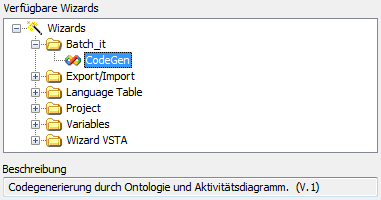
\includegraphics[width=0.7\textwidth]{graphics/implementation/wizards}
  \caption{Auswahl des zenon Wizards}
\end{figure}

\ac{VSTA} verfügt über ein Modul zum aufbauen und ändern von Benutzeroberflächen, welches ermöglicht mit recht geringem Aufwand eine Vielzahl an Interaktionselementen zu positionieren und falls benötigt auch Templates der Methoden zur Bearbeitung der vom Benutzer eingegebenen Daten generiert.

\begin{figure}[hbt!]
  \centering
  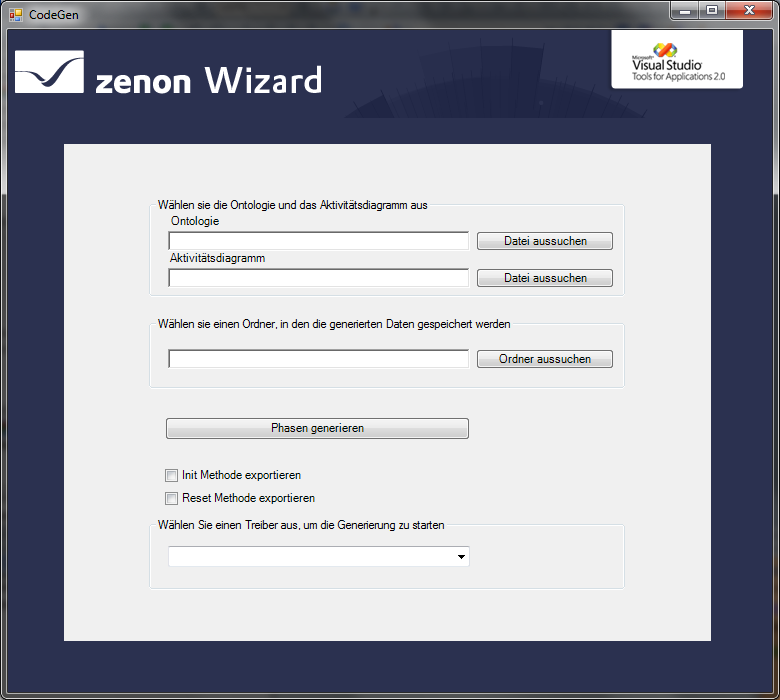
\includegraphics[width=0.8\textwidth]{graphics/implementation/wizard_final}
  \caption{Benutzeroberfläche für den Wizard}
\end{figure}

\newpage
\section{Zusammenfassung}
Vor eigentlicher Umsetzung des Aufbaus der Anlage wurde ein schematisches Modell erzeugt auf Basis dessen die Apperatur schlussendlich realisiert wurde. Um die Steuerung mehrerer Arbeitsschritte automatisieren zu können, wurden Prozeduren und Rezepte erstellt, mit Hilfe dieser das Zusammenfassen einzelner Grundfunktionen ermöglicht wurde. Über die Visualisierung der Anlage wurde neben der Möglichkeit der interaktiven Steuerung auch das Anzeigen von fallweise quittierungspflichten Alarmen integriert. Eine Ontologie diente als detailgetreues Abbild der Anlage. Verfügbare Funktionen und Wege wurden im Aktivitätsdiagramm definiert. Eine Kombination der beiden als XML exportierten Modelle ergab das Fundament der automatisierten Codegenerierung mittels eines selbst geschriebenen zenon Wizards.
